\documentclass[IB,BIB]{TFUOC}

% Paquetes de apoyo para tablas, enlaces y figuras.
\usepackage{amsmath}
\usepackage{booktabs}
\usepackage{longtable}
\usepackage{tabularx}
\usepackage{array}
\usepackage{float}
\usepackage[hidelinks]{hyperref}
\usepackage{doi}
\setlength{\headheight}{43pt}

% Datos del trabajo
\title{Identificación de biomarcadores transcriptómicos pronósticos y predictivos de respuesta a inmunoterapia en melanoma mediante análisis bioinformático integrativo}
\titcrt{Biomarcadores en melanoma}
\author{Sonia Salmerón Fructuoso}
\date{Mayo de 2026}

\nomPDC{Dra. Teresa Torres Moral}
\nomPRA{Pendiente de completar}
\titulac{Máster Universitario en Bioinformática y Bioestadística}
\area{Bioinformática traslacional y análisis transcriptómico}
\idioma{Castellano}
\credits{15}
\parcla{melanoma; inmunoterapia; biomarcadores; transcriptómica; RNA-seq; NanoString; GEO; TCGA}

\licenc{ccByNcNd}

\abstractidioma{
El melanoma avanzado es una neoplasia heterogénea en la que la inmunoterapia con inhibidores de checkpoint ha mejorado el pronóstico de un subgrupo de pacientes, aunque una proporción relevante no responde o desarrolla resistencia. Este trabajo plantea un análisis bioinformático integrativo para identificar biomarcadores transcriptómicos asociados al pronóstico y a la respuesta a inmunoterapia. El bloque pronóstico se basa en TCGA-SKCM, mientras que el bloque predictivo utiliza cohortes GEO con datos de expresión y respuesta clínica. Tras una fase inicial de integración multi-cohorte, el análisis predictivo se reorganizó en una estrategia de descubrimiento, validación y sensibilidad: GSE78220 como cohorte principal RNA-seq tumoral anti-PD-1, GSE215868 como validación tumoral anti-PD-1 en NanoString, GSE211645 como validación exploratoria anti-CTLA-4, GSE91061 como validación tumoral RNA-seq independiente y GSE94873 como sensibilidad en sangre periférica. Los resultados muestran una señal coherente relacionada con presentación antigénica MHC-I y respuesta a IFN-gamma, aunque limitada por tamaño muestral y diferencias de plataforma. La memoria documenta el diseño, la metodología reproducible y la interpretación crítica de estos resultados.
}

\abstractenglish{
Advanced melanoma is a heterogeneous malignancy in which immune checkpoint inhibitors have improved outcomes for a subset of patients, although many patients do not respond or develop resistance. This project proposes an integrative bioinformatics analysis to identify transcriptomic biomarkers associated with prognosis and response to immunotherapy. The prognostic block is based on TCGA-SKCM, whereas the predictive block uses GEO cohorts with gene expression and clinical response data. After an initial multi-cohort integration stage, the predictive analysis was reorganized into a discovery, validation and sensitivity framework: GSE78220 as the main tumor RNA-seq anti-PD-1 discovery cohort, GSE215868 as tumor anti-PD-1 NanoString validation, GSE211645 as exploratory anti-CTLA-4 validation, GSE91061 as independent tumor RNA-seq validation, and GSE94873 as peripheral blood sensitivity analysis. The results point to a biologically coherent signal related to MHC-I antigen presentation and IFN-gamma response, while being limited by sample size and platform heterogeneity. This report documents the study design, reproducible methodology and critical interpretation of the results.
}

\begin{document}

\estructura

\tableofcontents
\listoffigures
\listoftables

\chapter{Introducción}

\section{Contexto y justificación del trabajo}

El melanoma cutáneo es el tumor maligno de piel de mayor mortalidad y constituye un problema clínico relevante en estadios avanzados o metastásicos. La introducción de los inhibidores de checkpoint inmunológico, especialmente anti-PD-1 y anti-CTLA-4, ha modificado de forma sustancial el tratamiento de la enfermedad. Sin embargo, la respuesta clínica es heterogénea: una parte de los pacientes responde de forma duradera, mientras que otros no responden o desarrollan resistencia secundaria.

Esta heterogeneidad justifica la búsqueda de biomarcadores moleculares que ayuden a estratificar pacientes y a comprender los mecanismos asociados a respuesta o resistencia. La transcriptómica permite estudiar de forma global la actividad génica del tumor y de su microambiente, por lo que resulta especialmente adecuada para explorar firmas relacionadas con presentación antigénica, señalización de interferón, infiltración inmune y otros procesos relevantes en inmunoterapia.

El proyecto se plantea como un análisis bioinformático integrativo de datos públicos, combinando un bloque pronóstico basado en TCGA-SKCM y un bloque predictivo basado en cohortes GEO con datos de tratamiento y respuesta a inmunoterapia.

\section{Objetivos del trabajo}

\subsection{Objetivo general}

Identificar y evaluar biomarcadores transcriptómicos asociados al pronóstico y a la respuesta a inmunoterapia en melanoma mediante análisis bioinformático reproducible de cohortes públicas.

\subsection{Objetivos específicos}

\begin{itemize}
    \item Explorar la utilidad de TCGA-SKCM como cohorte pronóstica en melanoma.
    \item Construir y documentar objetos de análisis reproducibles para cohortes GEO con datos transcriptómicos y respuesta a inmunoterapia.
    \item Realizar un análisis principal de descubrimiento en GSE78220, cohorte tumoral RNA-seq tratada con anti-PD-1.
    \item Validar la dirección y transferibilidad de los genes candidatos en cohortes independientes tumorales y de sangre.
    \item Evaluar la consistencia de la señal en genes comunes entre plataformas, interpretando las limitaciones derivadas de RNA-seq y NanoString.
    \item Documentar el flujo de trabajo mediante R Markdown, objetos SummarizedExperiment, tablas de resultados y repositorio GitHub.
\end{itemize}

\section{Impacto en sostenibilidad, ético-social y de diversidad}
\label{s:etic}

Este trabajo utiliza exclusivamente datos públicos y anonimizados procedentes de repositorios reconocidos, principalmente GEO y TCGA \cite{GEO,TCGA}. Por tanto, no implica contacto directo con pacientes ni tratamiento de datos identificativos. El impacto ético-social se relaciona principalmente con la reutilización responsable de datos biomédicos, la reproducibilidad del análisis y la interpretación prudente de resultados exploratorios.

En relación con los Objetivos de Desarrollo Sostenible, el proyecto se alinea con el ODS 3 (salud y bienestar), al buscar biomarcadores que puedan contribuir a mejorar la selección de tratamientos en cáncer; con el ODS 9 (industria, innovación e infraestructura), por el desarrollo de un pipeline bioinformático reproducible; y con el ODS 17 (alianzas para lograr los objetivos), por basarse en ciencia abierta, datos públicos y herramientas de código abierto.

Desde la perspectiva de género y diversidad, el análisis no excluye muestras por sexo. En TCGA-SKCM la variable sexo está disponible y se podrá considerar como covariable en los modelos pronósticos. En cambio, las cohortes GEO del bloque predictivo no disponen de información de sexo armonizada en las variables actualmente utilizadas, lo que se documenta como limitación.

\section{Enfoque y método seguido}

El enfoque inicial integraba varias cohortes GEO en un único objeto común. Tras revisar las limitaciones metodológicas, especialmente la restricción a genes presentes en paneles NanoString y la mezcla de tejido tumoral, sangre y tratamientos distintos, el análisis predictivo se reorganizó en una arquitectura de descubrimiento, validación y sensibilidad.

La estrategia final separa el descubrimiento principal, realizado en GSE78220 por ser una cohorte tumoral RNA-seq anti-PD-1 con transcriptoma completo, de las validaciones en cohortes NanoString y de los análisis de sensibilidad en sangre. Esta decisión reduce el riesgo de mezclar mecanismos biológicos distintos y permite interpretar cada resultado en su contexto.

\section{Planificación del trabajo}

La planificación se ha adaptado a la evolución metodológica del proyecto. El bloque GEO se ha priorizado por su mayor complejidad técnica y biológica, mientras que el bloque TCGA se mantiene como análisis pronóstico paralelo. La memoria final integrará ambos bloques de forma diferenciada: pronóstico en TCGA-SKCM y predicción de respuesta en GEO.

\section{Breve sumario de productos obtenidos}

Hasta el momento se han generado objetos SummarizedExperiment por cohorte, informes HTML de exploración y análisis, tablas CSV de resultados, scripts R Markdown reproducibles y un repositorio GitHub actualizado:

\begin{center}
\url{https://github.com/Soniasalme/TFM_MELANOMA_INMUNOTERAPIA}
\end{center}

\section{Breve descripción de los otros capítulos}

El capítulo 2 resume el estado del arte biológico y computacional. El capítulo 3 describe los datos y la metodología. El capítulo 4 presenta los resultados del bloque predictivo y la estructura prevista del bloque pronóstico. El capítulo 5 discute la interpretación biológica y las limitaciones. El capítulo 6 resume conclusiones, planificación y líneas futuras.

\section{Declaración sobre el uso de inteligencia artificial generativa}

Durante el desarrollo del trabajo se ha utilizado inteligencia artificial generativa como apoyo para organizar ideas, revisar redacción, estructurar documentos, depurar scripts y preparar borradores de explicación metodológica. La selección de datos, ejecución de análisis, interpretación científica y validación final de los resultados recaen íntegramente en la estudiante. Los contenidos generados con ayuda de IA han sido revisados críticamente y contrastados con los datos, scripts y recomendaciones de la tutora. Esta utilización se declara de forma explícita por transparencia académica y no sustituye la autoría ni la responsabilidad intelectual del trabajo.

\chapter{Estado del arte}

\section{El melanoma: biología y clasificación molecular}

El melanoma es la neoplasia maligna de mayor mortalidad entre los tumores cutáneos. Su incidencia ha aumentado de forma sostenida, especialmente en poblaciones caucásicas con exposición solar acumulada \cite{Potrony2015}. Aunque en estadios localizados puede tratarse quirúrgicamente, el melanoma metastásico presenta un comportamiento clínico agresivo y, hasta la aparición de las terapias modernas, la mediana de supervivencia global era de 6--9 meses \cite{Lebbe2014}.

Desde el punto de vista molecular, el melanoma no es una enfermedad unitaria sino un conjunto de subtipos biológicamente distintos \cite{Bastian2014}. La clasificación más aceptada distingue cuatro subtipos principales según el patrón de mutaciones somáticas: mutante en \textit{BRAF}, mutante en \textit{NRAS}, mutante en \textit{NF1} y triple salvaje. El subtipo \textit{BRAF}$^{V600E}$ es el más frecuente (aproximadamente el 50\,\% de los melanomas cutáneos) y se caracteriza por una activación constitutiva de la vía MAPK, lo que hace que sea el principal objetivo de las terapias dirigidas con inhibidores de BRAF/MEK \cite{Bastian2014, Switzer2022}. Los subtipos \textit{NRAS} y \textit{NF1} también activan la vía MAPK por mecanismos alternativos, mientras que los melanomas triple salvaje son molecularmente más heterogéneos \cite{Podlipnik2021}.

Además de las mutaciones somáticas, existe una predisposición genética relevante. Los genes de alta penetrancia para melanoma incluyen \textit{CDKN2A} (presente en alrededor del 20\,\% de las familias con melanoma), \textit{CDK4}, \textit{BAP1} y \textit{TERT}, mientras que los genes de penetrancia moderada incluyen \textit{MC1R} y \textit{MITF} \cite{Potrony2015}. La carga mutacional tumoral (\textit{tumor mutational burden}, TMB) es un factor adicional de relevancia, ya que se ha asociado al beneficio clínico de los inhibidores de checkpoint inmunológico (ICI) en varios estudios \cite{Podlipnik2021}.

\section{Inhibidores de checkpoint inmunológico: mecanismos de acción}

Los inhibidores de checkpoint inmunológico constituyen la principal estrategia de inmunoterapia en melanoma avanzado. Su fundamento biológico reside en el papel regulador de las moléculas CTLA-4 y PD-1 en el mantenimiento de la tolerancia periférica de los linfocitos T \cite{FifeBluestone2008}.

CTLA-4 (CD152) es un receptor inhibidor expresado en la superficie de las células T que compite con CD28 por la unión a los ligandos B7-1 y B7-2 en las células presentadoras de antígeno. La unión de CTLA-4 reduce la amplitud de la respuesta T en las fases iniciales de activación en el ganglio linfático. PD-1 (CD279), por su parte, actúa principalmente en el lugar tumoral: al unirse a sus ligandos PD-L1 (B7-H1) y PD-L2 (B7-DC), suprime la función efectora de las células T que reconocen el tumor \cite{FifeBluestone2008}. Esta diferencia en el sitio de acción ---nódulo linfático para CTLA-4 y microambiente tumoral para PD-1--- tiene consecuencias sobre el perfil de toxicidad y la biología de la respuesta \cite{Dempke2017}.

Los anticuerpos monoclonales que bloquean estos receptores eliminan los frenos inmunológicos, permitiendo que el sistema inmune reconozca y elimine las células tumorales. Ipilimumab (anti-CTLA-4) fue el primero en demostrar beneficio de supervivencia en melanoma avanzado. Los anti-PD-1, especialmente pembrolizumab y nivolumab, han mostrado mayor eficacia con menor toxicidad y se han convertido en el estándar de primera línea \cite{Switzer2022}.

\section{Evidencia clínica de los inhibidores de checkpoint en melanoma}

\subsection{Anti-PD-1: pembrolizumab y nivolumab}

Hamid et al.\ demostraron por primera vez la actividad de pembrolizumab (entonces denominado lambrolizumab o MK-3475) en melanoma avanzado en un ensayo de fase I con 135 pacientes \cite{Hamid2013}. La tasa de respuesta confirmada fue del 38\,\% en el conjunto de dosis, llegando al 52\,\% en el grupo que recibió 10\,mg/kg cada 2 semanas. Las respuestas fueron duraderas (mediana de 11 meses de seguimiento) y el perfil de toxicidad fue predominantemente de grado 1--2.

Robert et al.\ extendieron estos hallazgos en el estudio KEYNOTE-001, evaluando pembrolizumab en pacientes con melanoma avanzado refractario a ipilimumab \cite{Robert2014}. En esta cohorte de 173 pacientes, la tasa de respuesta global fue del 26\,\% tanto a 2\,mg/kg como a 10\,mg/kg cada 3 semanas, con un perfil de toxicidad manejable. Estos datos establecieron pembrolizumab como una opción eficaz incluso en pacientes previamente tratados con anti-CTLA-4.

\subsection{Anti-CTLA-4: ipilimumab}

Ipilimumab fue aprobado en 2011 tras demostrar beneficio de supervivencia en dos ensayos de fase III. Un análisis agrupado de datos de supervivencia global de 10 estudios prospectivos y dos retrospectivos, incluyendo 1.861 pacientes, mostró una mediana de supervivencia global de 11,4 meses (IC 95\,\%: 10,7--12,1) y una tasa de supervivencia a 3 años del 22\,\%, con una meseta que se inicia alrededor del tercer año de seguimiento y se mantiene hasta los 10 años de observación \cite{Schadendorf2015}. Esta meseta de supervivencia representa uno de los hallazgos más relevantes en el campo y constituye la base para hablar de respuestas duraderas.

Con un seguimiento de 5--6 años, Lebb\'e et al.\ confirmaron que la supervivencia a 5 años con ipilimumab alcanza entre el 12,3\,\% y el 28,4\,\% según la dosis y el estado de tratamiento previo \cite{Lebbe2014}. Este seguimiento prolongado refuerza el concepto de beneficio a largo plazo en un subgrupo de pacientes.

\subsection{Nuevas combinaciones y resistencia}

A pesar de los avances, solo el 25\,\% de los pacientes responde de forma sostenida a la inmunoterapia, y los mecanismos de resistencia primaria y secundaria representan un reto clínico y biológico. Entre los mecanismos descritos se encuentran el agotamiento de células T, la sobreexpresión de caspasa-8 y $\beta$-catenina, la amplificación de los genes PD-L1/PD-L2 y las mutaciones en MHC-I/II \cite{Dempke2017}. Para superar estas resistencias, se evalúan moléculas de segunda y tercera generación dirigidas a nuevas dianas, como TIM-3, LAG-3, VISTA, IDO y KIR, así como anticuerpos coestimuladores como anti-CD40, anti-GITR, anti-OX40 y anti-ICOS \cite{Dempke2017}.

Kim et al.\ exploraron la combinación de ceralasertib (un inhibidor de ATR, enzima clave en la respuesta al daño en el ADN) con durvalumab (anti-PD-L1) en 30 pacientes con melanoma refractario a anti-PD-1 \cite{Kim2022}. La tasa de respuesta objetiva fue del 31\,\% y la tasa de control de la enfermedad del 63,3\,\%, con una duración mediana de respuesta de 8,8 meses. Este estudio subraya el potencial de combinar inmunoterapia con agentes que modulan la reparación del ADN para superar la resistencia.

Una visión de conjunto del panorama terapéutico actual, incluyendo quimioterapia, terapias dirigidas BRAF/MEK, inmunoterapia y terapias combinadas, se puede encontrar en las revisiones de Switzer et al.\ \cite{Switzer2022} y Dhanyamraju y Patel \cite{Dhanyamraju2022}.

\section{Biomarcadores transcriptómicos: pronóstico y predicción}

La identificación de biomarcadores moleculares capaces de estratificar pacientes antes del tratamiento es uno de los objetivos centrales de la oncología de precisión. Se distinguen dos tipos: los biomarcadores pronósticos, que informan sobre la evolución de la enfermedad independientemente de la terapia, y los biomarcadores predictivos, que se asocian a la probabilidad de respuesta a un tratamiento específico.

TCGA-SKCM constituye la cohorte de referencia para el estudio pronóstico en melanoma, al reunir datos de expresión génica, variantes somáticas, metilación y datos clínicos de supervivencia en centenares de pacientes \cite{DasTCGA2020, TCGA}. Los marcadores genéticos de peor pronóstico identificados incluyen mutaciones en \textit{CDKN2A}, amplificaciones de \textit{TERT} y alta carga de daño UV, entre otros \cite{Podlipnik2021}.

En cuanto a la predicción de respuesta a ICI, los factores más estudiados son la expresión de PD-L1, la TMB, la presencia de células T infiltrantes y la firma de IFN-$\gamma$ \cite{Hamid2013, Robert2014}. La transcriptómica de alto rendimiento permite estudiar estos marcadores de forma global y generar firmas multigénicas con potencial predictivo. Sin embargo, su extrapolación entre plataformas (RNA-seq vs.\ NanoString) y tejidos (tumor vs.\ sangre periférica) constituye un reto técnico importante que este trabajo aborda de forma explícita.

\section{Integración de cohortes ómicas}

La disponibilidad de repositorios públicos como GEO y TCGA ha facilitado el análisis de múltiples cohortes con datos de expresión génica y respuesta clínica \cite{GEO, DasTCGA2020}. Sin embargo, la integración directa de cohortes procedentes de plataformas distintas (RNA-seq y NanoString), tejidos diferentes (tumor y sangre periférica) y tratamientos heterogéneos (anti-PD-1 y anti-CTLA-4) introduce riesgos metodológicos relevantes: mezcla de efectos biológicos, restricción al subconjunto de genes comunes y pérdida de potencia estadística.

Por ello, el diseño de este trabajo adopta una arquitectura de descubrimiento, validación y sensibilidad que separa explícitamente las cohortes según su tejido, plataforma y tipo de tratamiento. Esta estrategia, coherente con las recomendaciones metodológicas de la literatura, permite interpretar cada resultado en su contexto biológico y técnico apropiado.

\section{Hipótesis de trabajo}

A partir del estado del arte descrito, la hipótesis central de este proyecto es que los pacientes con melanoma avanzado respondedores a inmunoterapia presentan una señal transcriptómica diferencial relacionada con la activación del sistema inmune, la presentación antigénica por MHC-I y la señalización de IFN-$\gamma$. Esta señal, identificable en el transcriptoma tumoral completo mediante RNA-seq, puede ser evaluada ---con limitaciones derivadas de la distancia biológica y técnica--- en cohortes de validación con otras plataformas, tejidos o tipos de checkpoint.

\chapter{Metodología}

\section{Diseño general del estudio}

El proyecto se organiza en dos bloques. El primero es un bloque pronóstico basado en TCGA-SKCM \cite{TCGA}. El segundo es un bloque predictivo basado en cohortes GEO \cite{GEO} con datos de expresión y respuesta a inmunoterapia. Este capítulo describe principalmente el bloque GEO, que constituye el desarrollo metodológico más avanzado hasta el momento.

\section{Cohortes utilizadas}

\begin{table}[H]
\centering
\caption{Cohortes GEO utilizadas en el bloque predictivo. Los tratamientos anti-PD-1 incluyen pembrolizumab y nivolumab \cite{Hamid2013,Robert2014}; el tratamiento anti-CTLA-4 es tremelimumab (análogo a ipilimumab) \cite{Schadendorf2015,Lebbe2014}.}
\label{tab:cohortes_geo}
\begin{tabularx}{\textwidth}{l l l l l}
\toprule
Cohorte & Tejido & Plataforma & Tratamiento & Rol \\
\midrule
GSE78220 \cite{GSE78220}   & Tumor       & RNA-seq    & anti-PD-1                & Descubrimiento \\
GSE215868 \cite{GSE215868} & Tumor       & NanoString & anti-PD-1                & Validación tumoral \\
GSE211645 \cite{GSE211645} & Tumor       & NanoString & anti-CTLA-4              & Validación exploratoria \\
GSE91061 \cite{GSE91061}   & Sangre/PBMC & RNA-seq    & varios ICI               & Sensibilidad \\
GSE94873 \cite{GSE94873}   & Sangre      & NanoString & tremelimumab (anti-CTLA-4) & Sensibilidad \\
\bottomrule
\end{tabularx}
\end{table}

\section{Preprocesamiento y objetos de análisis}

Para cada cohorte se construyó un objeto SummarizedExperiment con matriz de expresión, metadatos clínicos y anotación génica. Se verificó la coherencia entre columnas de la matriz y filas del colData, se recodificó la variable de respuesta binaria y se documentaron las muestras pretratamiento. En GSE78220 se aplicó transformación log2(expr + 1) antes del análisis diferencial.

\section{Verificación de escala y preprocesamiento por cohorte}

Antes del análisis diferencial se verificó explícitamente la escala de cada cohorte para evitar dobles transformaciones. GSE78220 contiene valores FPKM en escala lineal (rango 0--8\,M), por lo que se aplica $\log_2(\text{FPKM}+1)$ antes del modelo \textit{limma}. Las cohortes de validación (GSE215868, GSE211645) y de sensibilidad (GSE91061 en escala RLD, GSE94873 en NanoString normalizado) ya están en escala razonablemente normalizada y pueden contener valores negativos, por lo que \textbf{no} se les aplica ninguna transformación logarítmica adicional. En GSE78220 se realizó además un filtrado de baja expresión: se retienen únicamente los genes con FPKM $\geq 1$ en al menos el 20\,\% de las muestras (mínimo 5), lo que reduce el espacio de genes de 25.268 a 14.549. Este criterio está inspirado en el uso de \texttt{filterByExpr} de edgeR en datos de recuentos crudos, adaptado aquí a la escala FPKM al no disponer de recuentos originales.

\section{Control de calidad previo al análisis diferencial}

Para cada cohorte se generaron gráficos de control de calidad: boxplot de la distribución de expresión por muestra y análisis de componentes principales (PCA) coloreado por respuesta, siguiendo el estándar de las prácticas de análisis de datos ómicos \cite{Lawrence2013}. La homogeneidad de las distribuciones y la ausencia de muestras atípicas se verificaron antes de proceder al análisis diferencial. Los resultados del PCA y las puntuaciones por muestra se exportaron como ficheros CSV para trazabilidad. Al final de cada informe se incluye \texttt{sessionInfo()} para garantizar la reproducibilidad computacional.

\section{Análisis diferencial}

El análisis diferencial entre respondedores y no respondedores se realizó con limma \cite{Smyth2004, Ritchie2015}. En el análisis principal de GSE78220 \cite{GSE78220} se utilizó el transcriptoma filtrado (14.549 genes), evitando la restricción a genes presentes en paneles NanoString. Para las cohortes de validación, se evaluó el solapamiento de genes candidatos y la dirección del efecto. El análisis incluye volcano plot, MA plot y heatmap de los genes nominales más significativos para una inspección visual completa de los resultados.

\section{Modelos predictivos exploratorios}

Se construyó un score de firma basado en genes seleccionados dentro de cada iteración de validación leave-one-out cross-validation (LOOCV), con el objetivo de evitar filtración de información entre entrenamiento y test. El área bajo la curva ROC (AUC) se utilizó como métrica principal por su robustez relativa ante desbalance de clases.

\section{Validación, sensibilidad y consistencia}

GSE215868 \cite{GSE215868} se utilizó como validación tumoral anti-PD-1 en plataforma NanoString. GSE211645 \cite{GSE211645} se trató como validación exploratoria en otro checkpoint, no como validación directa de anti-PD-1. GSE91061 \cite{GSE91061} y GSE94873 \cite{GSE94873} se analizaron como sensibilidad en sangre. Finalmente, el dataset integrado tumoral de 200 genes comunes se conservó para evaluar consistencia de dirección de efecto entre cohortes.

\section{Anotación funcional y análisis de sobrerrepresentación}

Una vez identificados los genes asociados a la supervivencia mediante el screening Cox, se realiza su anotación funcional en dos pasos. Primero, los identificadores Ensembl (formato de salida de TCGA-RNA-seq) se convierten a símbolo génico y Entrez ID mediante el paquete de Bioconductor \texttt{org.Hs.eg.db} \cite{Lawrence2013}, eliminando previamente el número de versión del identificador (e.g., \texttt{ENSG00000162645.13} $\to$ \texttt{ENSG00000162645}). Segundo, se aplica un análisis de sobrerrepresentación (ORA, \textit{Over-Representation Analysis}) sobre los genes con FDR $< 0{,}05$, separando genes protectores (HR $< 1$) y genes de riesgo (HR $> 1$). El ORA se ejecuta sobre la ontología GO-BP (\textit{Gene Ontology, Biological Process}) mediante la función \texttt{enrichGO} de \texttt{clusterProfiler} \cite{clusterProfiler2012}, con el universo de genes testados como referencia y corrección de Benjamini-Hochberg. Este paso proporciona la base funcional para la interpretación biológica de la firma transcriptómica pronóstica.

\section{Reproducibilidad}

Todos los análisis se documentaron mediante R Markdown y se guardaron tablas CSV de resultados. El repositorio GitHub del proyecto se utiliza como mecanismo de control de versiones y trazabilidad:

\begin{center}
\url{https://github.com/Soniasalme/TFM_MELANOMA_INMUNOTERAPIA}
\end{center}

\chapter{Resultados}

\section{Descubrimiento en GSE78220}

El análisis principal se realizó en GSE78220 (25 muestras, tumor, RNA-seq, anti-PD-1). Tras verificar que los datos están en escala FPKM lineal, se aplicó la transformación $\log_2(\text{FPKM}+1)$ y se realizó un filtrado explícito de baja expresión: se eliminaron los genes con FPKM $< 1$ en al menos 5 muestras (20\,\% del total), lo que redujo el transcriptoma de 25.268 genes originales a \textbf{14.549 genes testados} (Tabla~\ref{tab:qc_gse78220}). No se detectaron genes significativos tras corrección FDR, resultado esperable por el tamaño muestral. Se identificaron \textbf{539 genes nominales} ($p < 0{,}05$, $|logFC| \geq 0{,}5$) como candidatos exploratorios.

\begin{table}[H]
\centering
\caption{Control de calidad y filtrado en GSE78220.}
\label{tab:qc_gse78220}
\begin{tabularx}{\textwidth}{l r}
\toprule
Paso de filtrado & Genes \\
\midrule
Genes/filas originales & 25.268 \\
Retirados por varianza cero & 2.663 \\
Retirados por baja expresión (FPKM $< 1$ en $<$5 muestras) & 10.719 \\
\textbf{Genes retenidos para DEA} & \textbf{14.549} \\
\bottomrule
\end{tabularx}
\end{table}

El análisis de control de calidad incluyó un boxplot de distribuciones de expresión por muestra y un PCA coloreado por respuesta. Las distribuciones son homogéneas entre muestras y el PCA muestra cierta separación entre respondedores y no respondedores en PC1, aunque con solapamiento, coherente con la señal débil esperable dado el tamaño muestral.

\begin{table}[H]
\centering
\caption{Resumen del análisis de descubrimiento en GSE78220.}
\label{tab:discovery_gse78220}
\begin{tabularx}{\textwidth}{l l X}
\toprule
Resultado & Valor & Interpretación \\
\midrule
Muestras & 25 & Tamaño muestral reducido; análisis exploratorio. \\
Genes testados (tras QC) & 14.549 & Transcriptoma filtrado por FPKM y varianza. \\
Genes FDR $< 0{,}05$ & 0 & Compatible con baja potencia ($n=25$). \\
Genes nominales & 539 & Candidatos exploratorios para validación. \\
LOOCV — top 5 genes & AUC\,=\,0{,}853 & Señal exploratoria; no rendimiento clínico validado. \\
LOOCV — top 10 genes & AUC\,=\,0{,}686 & Disminuye al aumentar genes; patrón esperable. \\
\bottomrule
\end{tabularx}
\end{table}

El modelo predictivo exploratorio LOOCV alcanza su mejor rendimiento con una firma de \textbf{5 genes} (AUC $= 0{,}853$, exactitud $= 76\,\%$), lo que sugiere que un pequeño subconjunto de genes concentra la señal predictiva. Al aumentar el número de genes la AUC disminuye (top 10: AUC $= 0{,}686$; top 20: AUC $= 0{,}558$), patrón coherente con la inclusión de genes con menor señal real.

\subsection{Enriquecimiento funcional exploratorio en GSE78220}

Dado que ningún gen alcanzó significación estadística tras corrección FDR en el DEA principal (resultado esperable con $n=25$), el enriquecimiento funcional se realizó sobre los \textbf{539 genes nominales} ($p < 0{,}05$) como conjunto exploratorio. La ORA GO-BP (umbral de significación $p_{\text{adj}} < 0{,}10$) debe interpretarse en este contexto: no refleja genes validados estadísticamente, sino tendencias biológicas observadas en la muestra de descubrimiento. Se separaron genes con mayor expresión en respondedores (\textit{up in R}) y en no respondedores (\textit{down in R}). Los resultados más relevantes se presentan en la Tabla~\ref{tab:ora_gse78220}.

\begin{table}[H]
\centering
\caption{Principales términos GO-BP enriquecidos en el análisis de descubrimiento exploratorio (GSE78220). \textit{Down in R}: más expresados en no respondedores; \textit{Up in R}: más expresados en respondedores.}
\label{tab:ora_gse78220}
\begin{tabularx}{\textwidth}{l l r r}
\toprule
Dirección & Término GO-BP & FDR & $n$ genes \\
\midrule
\textit{Down in R} & Extracellular matrix organization & $1{,}2\times10^{-22}$ & 44 \\
\textit{Down in R} & Angiogenesis & $9{,}1\times10^{-12}$ & 43 \\
\textit{Down in R} & Collagen fibril organization & $2{,}8\times10^{-9}$ & 15 \\
\textit{Down in R} & VEGFR signaling pathway & $8{,}6\times10^{-8}$ & 16 \\
\textit{Down in R} & Connective tissue development & $1{,}6\times10^{-6}$ & 23 \\
\midrule
\textit{Up in R} & Amino acid catabolic process & 0{,}033 & 8 \\
\textit{Up in R} & Respiratory electron transport chain & 0{,}033 & 8 \\
\textit{Up in R} & Cytoplasmic translation & 0{,}033 & 10 \\
\bottomrule
\end{tabularx}
\end{table}

Los genes más altos en no respondedores están fuertemente enriquecidos en remodelación de la matriz extracelular (MEC), angiogénesis y activación estromal (colágenos, metaloproteasas, PDGFR, VEGFC), lo que apunta a un fenotipo mesenquimal-estromal asociado a resistencia a inmunoterapia. Los genes con mayor expresión en respondedores se asocian a metabolismo mitocondrial y síntesis proteica, coherentes con un microambiente tumoral metabólicamente activo e inmunológicamente competente.

\section{Validación tumoral}

La validación de los genes candidatos en las cohortes tumorales NanoString mostró solapamiento limitado, esperable por las diferencias de plataforma. En GSE215868 (105 muestras, NanoString, anti-PD-1), \textbf{6 de los top 50 genes} de descubrimiento estaban presentes en el panel y el 66{,}7\,\% mantuvo la misma dirección de efecto; la AUC de la firma fue de 0{,}547. En GSE211645 (40 muestras, NanoString, anti-CTLA-4), únicamente 1 gen solapó, por lo que se interpreta como generalización exploratoria a otro checkpoint y no como validación directa.

\begin{table}[H]
\centering
\caption{Resumen de la validación tumoral. La firma se calculó con los top 100 genes de GSE78220 presentes en cada panel.}
\label{tab:validacion_tumoral}
\begin{tabularx}{\textwidth}{l r r r r X}
\toprule
Cohorte & $n$ & NR/R & Solapam. top 50 & Dir. concord. & AUC \\
\midrule
GSE215868 & 105 & 59/45 & 6 genes & 66{,}7\,\% & 0{,}547 \\
GSE211645 & 40 & 28/12 & 1 gen & --- & 0{,}390 \\
\bottomrule
\end{tabularx}
\end{table}

\section{Sensibilidad en sangre}

La firma tumoral anti-PD-1 no mostró señal predictiva en sangre periférica. GSE91061 (51 muestras, RNA-seq, varios ICI) alcanzó AUC $= 0{,}474$ con 19 genes de la firma disponibles. GSE94873 (360 muestras, NanoString, anti-CTLA-4) alcanzó AUC $= 0{,}475$ con \textbf{solo 4 genes de firma con solapamiento} en el panel de 162 sondas; este resultado debe interpretarse con extrema prudencia: con únicamente 4 genes, el score de firma no puede considerarse una evaluación representativa de la firma original y el análisis tiene valor exclusivamente como sensibilidad exploratoria, no como validación formal. Ambos resultados son coherentes con la distancia biológica (tumor vs.\ sangre) y técnica (plataforma, checkpoint) entre las cohortes.

\begin{table}[H]
\centering
\caption{Análisis de sensibilidad en sangre. NR: no respondedores; R: respondedores.}
\label{tab:sensibilidad_sangre}
\begin{tabularx}{\textwidth}{l r r r r X}
\toprule
Cohorte & $n$ & NR/R & Genes firma & AUC & Distancia \\
\midrule
GSE91061 & 51 & 39/10 & 19 & 0{,}474 & Tumor→sangre; multi-ICI \\
GSE94873 & 360 & 314/46 & 4 & 0{,}475 & Tumor→sangre; anti-CTLA-4; NanoString \\
\bottomrule
\end{tabularx}
\end{table}

\section{Consistencia integrada en genes comunes}

El análisis de consistencia en 200 genes comunes entre cohortes tumorales identificó 69 genes concordantes en las tres cohortes, 61 con efecto positivo y 8 con efecto negativo. La señal más coherente se relacionó con presentación antigénica por MHC-I y respuesta a IFN-gamma.

\begin{table}[H]
\centering
\caption{Consistencia multi-cohorte en genes comunes.}
\label{tab:consistencia}
\begin{tabularx}{\textwidth}{l l}
\toprule
Resultado & Valor \\
\midrule
Genes comunes evaluados & 200 \\
Genes up en las tres cohortes & 61 \\
Genes down en las tres cohortes & 8 \\
Genes discordantes & 131 \\
Genes destacados & HLA-A/B/C/E/F, PSMB8, IFNGR1, STAT2, SLAMF7, ICAM1 \\
\bottomrule
\end{tabularx}
\end{table}

\section{Bloque pronóstico TCGA-SKCM}

El bloque pronóstico se basa en TCGA-SKCM \cite{TCGA}, cohorte de referencia en melanoma cutáneo. Su objetivo es identificar variables clínicas y transcriptómicas asociadas a la supervivencia global, de forma independiente al bloque predictivo. TCGA no contiene información homogénea de tratamiento con inmunoterapia ni respuesta clínica binaria, por lo que su análisis se centra en el pronóstico.

\subsection{Descripción de la cohorte}

La descarga mediante TCGAbiolinks proporcionó datos clínicos de 470 pacientes con 90 variables. Las variables de supervivencia se construyeron del siguiente modo: \texttt{OS\_event} = 1 si \texttt{vital\_status = Dead}, 0 si \texttt{vital\_status = Alive}; \texttt{OS\_time} se obtuvo de \texttt{days\_to\_death} en pacientes fallecidos y de \texttt{days\_to\_last\_follow\_up} en los censurados. Tras excluir casos con tiempo negativo o variables ausentes, el conjunto de datos válido para el análisis de supervivencia quedó integrado por 470 pacientes.

\subsection{Curvas de Kaplan-Meier}

Se generaron curvas de Kaplan-Meier globales y por subgrupos. La curva de supervivencia global muestra un descenso progresivo a lo largo del seguimiento, con una mediana de supervivencia estimada en torno a los 2--3 años (Figura~\ref{fig:km_global}).

\begin{figure}[H]
\centering
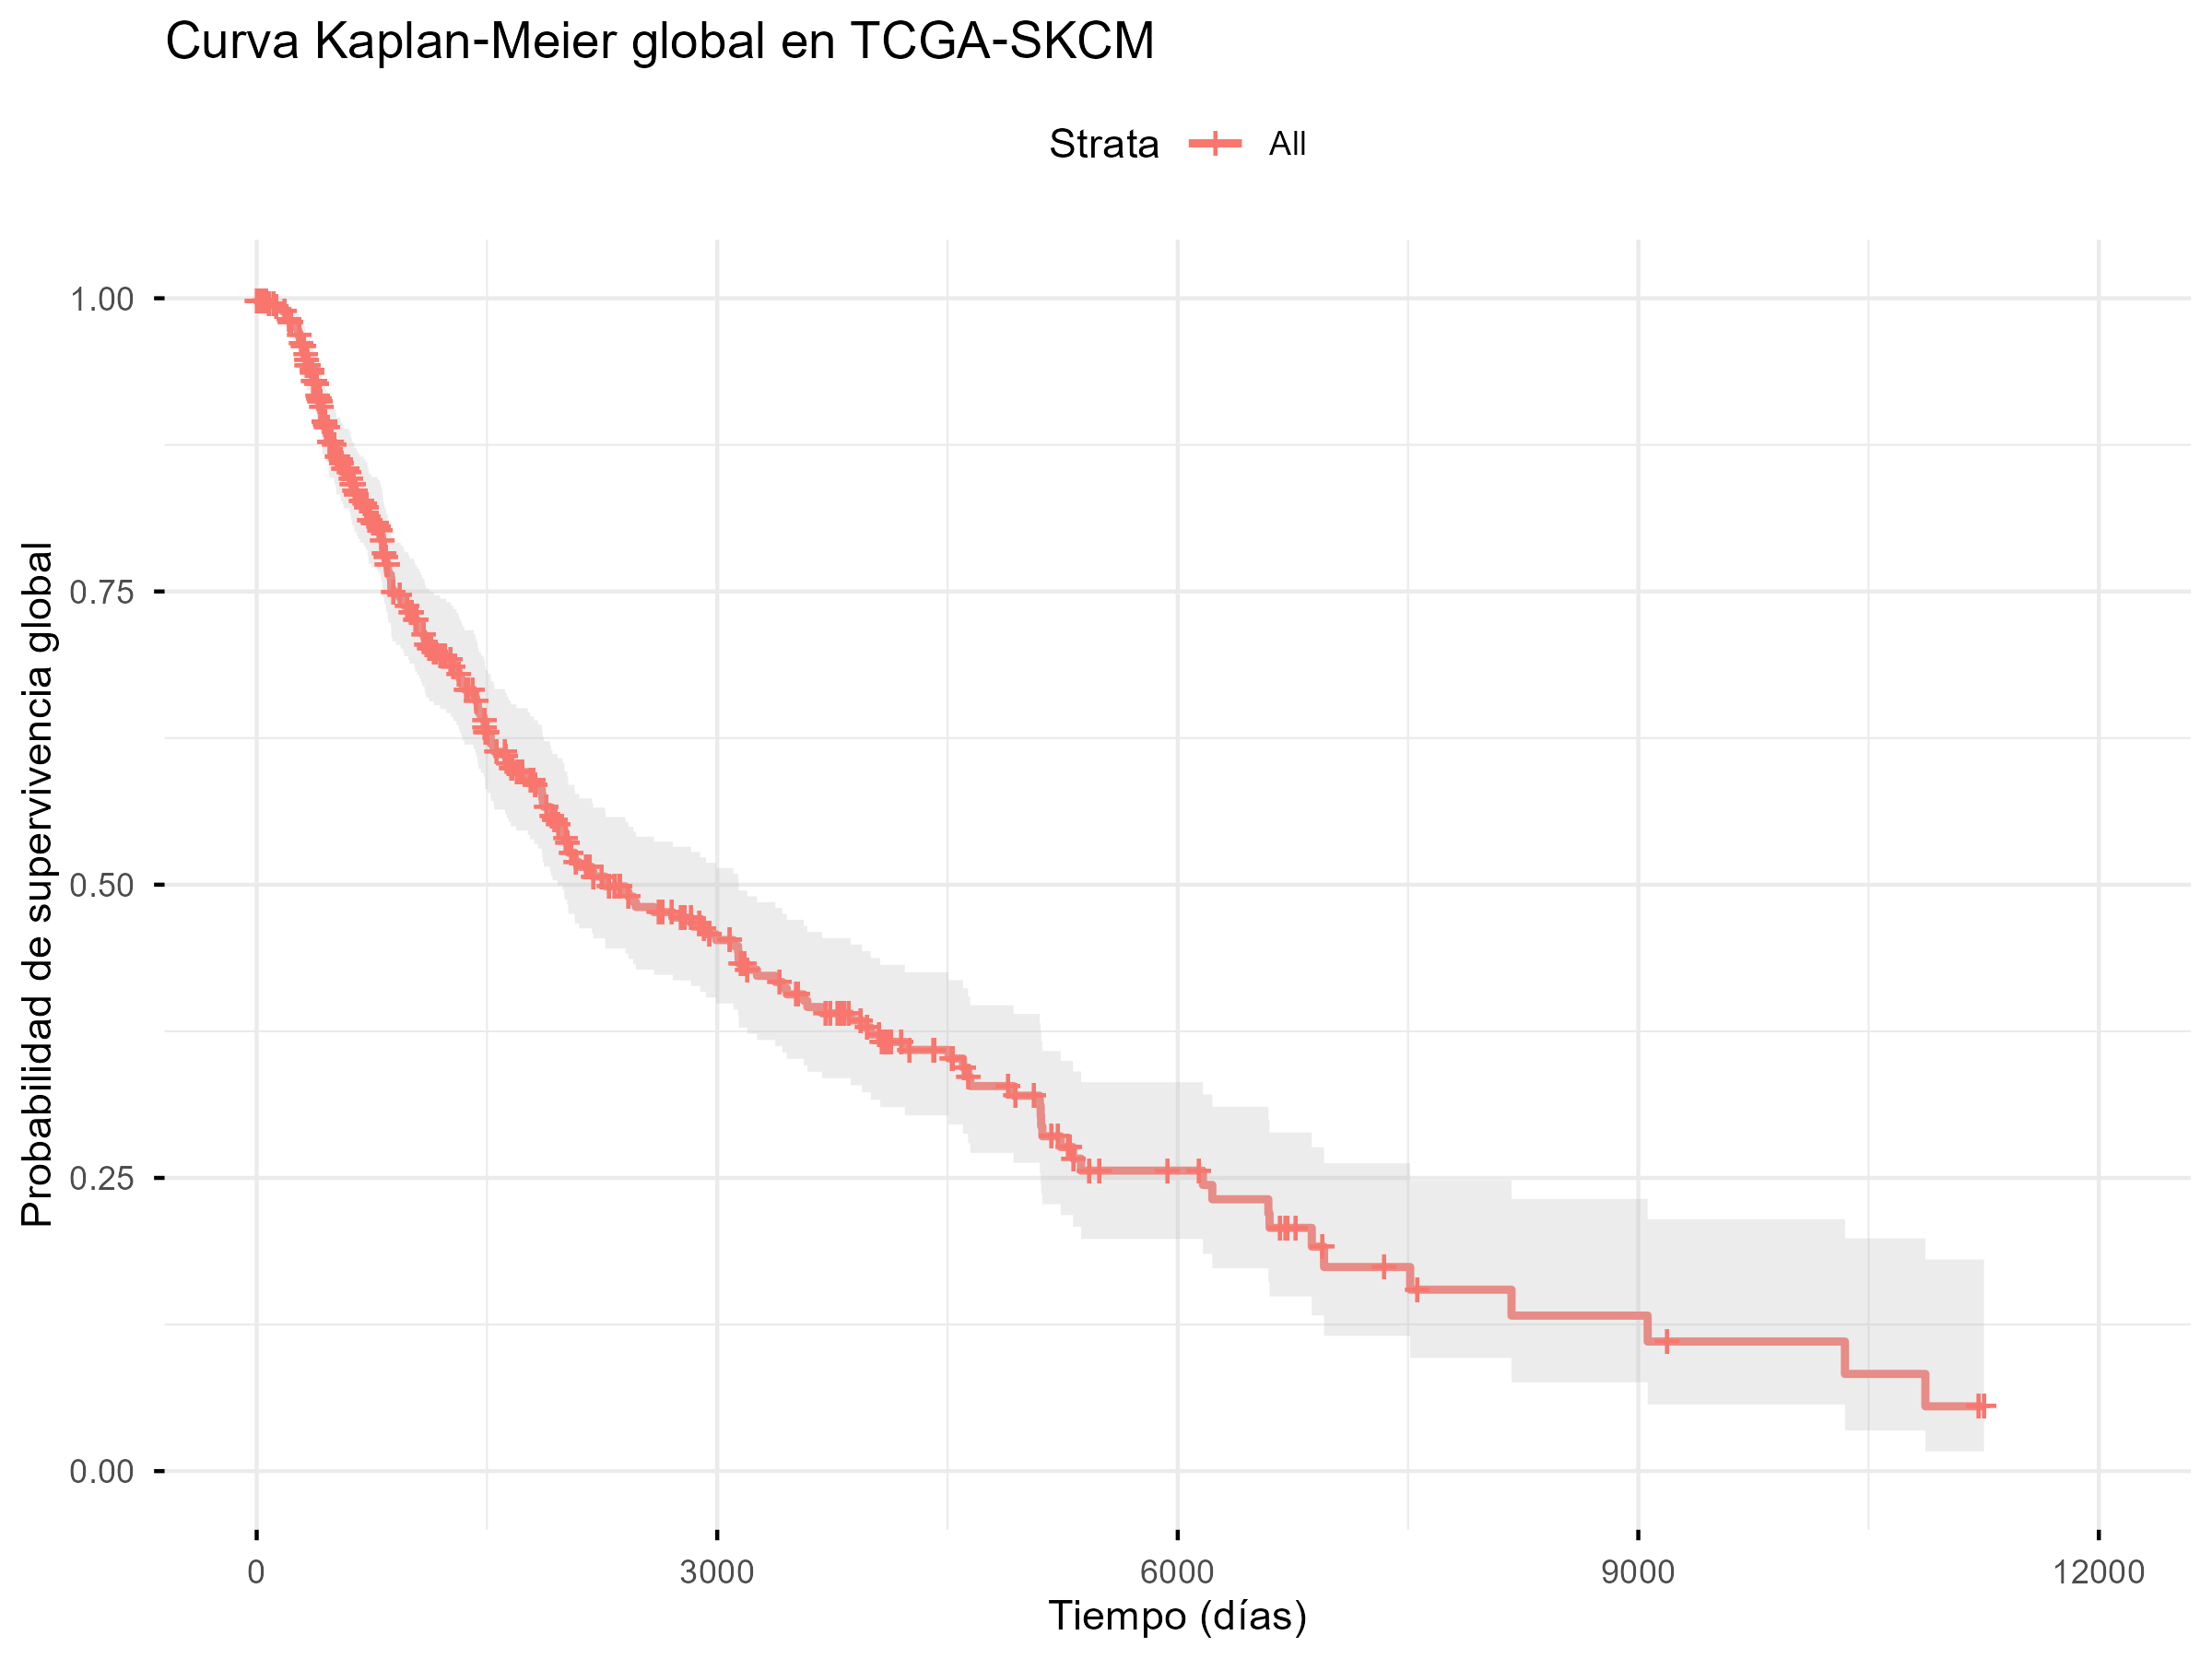
\includegraphics[width=0.85\textwidth]{figures/km_global_plot}
\caption{Curva de Kaplan-Meier de supervivencia global en TCGA-SKCM (N\,=\,470).}
\label{fig:km_global}
\end{figure}

El análisis por sexo no mostró diferencias estadísticamente significativas mediante el test log-rank, resultado coherente con los modelos Cox (Figura~\ref{fig:km_sexo_estadio}). Por el contrario, el análisis por estadio AJCC evidenció una separación progresiva de las curvas conforme aumenta el estadio, con peor pronóstico en estadio IV, confirmando la validez del sistema de estadificación como marcador pronóstico en esta cohorte.

\begin{figure}[H]
\centering
\begin{minipage}[t]{0.48\textwidth}
  \centering
  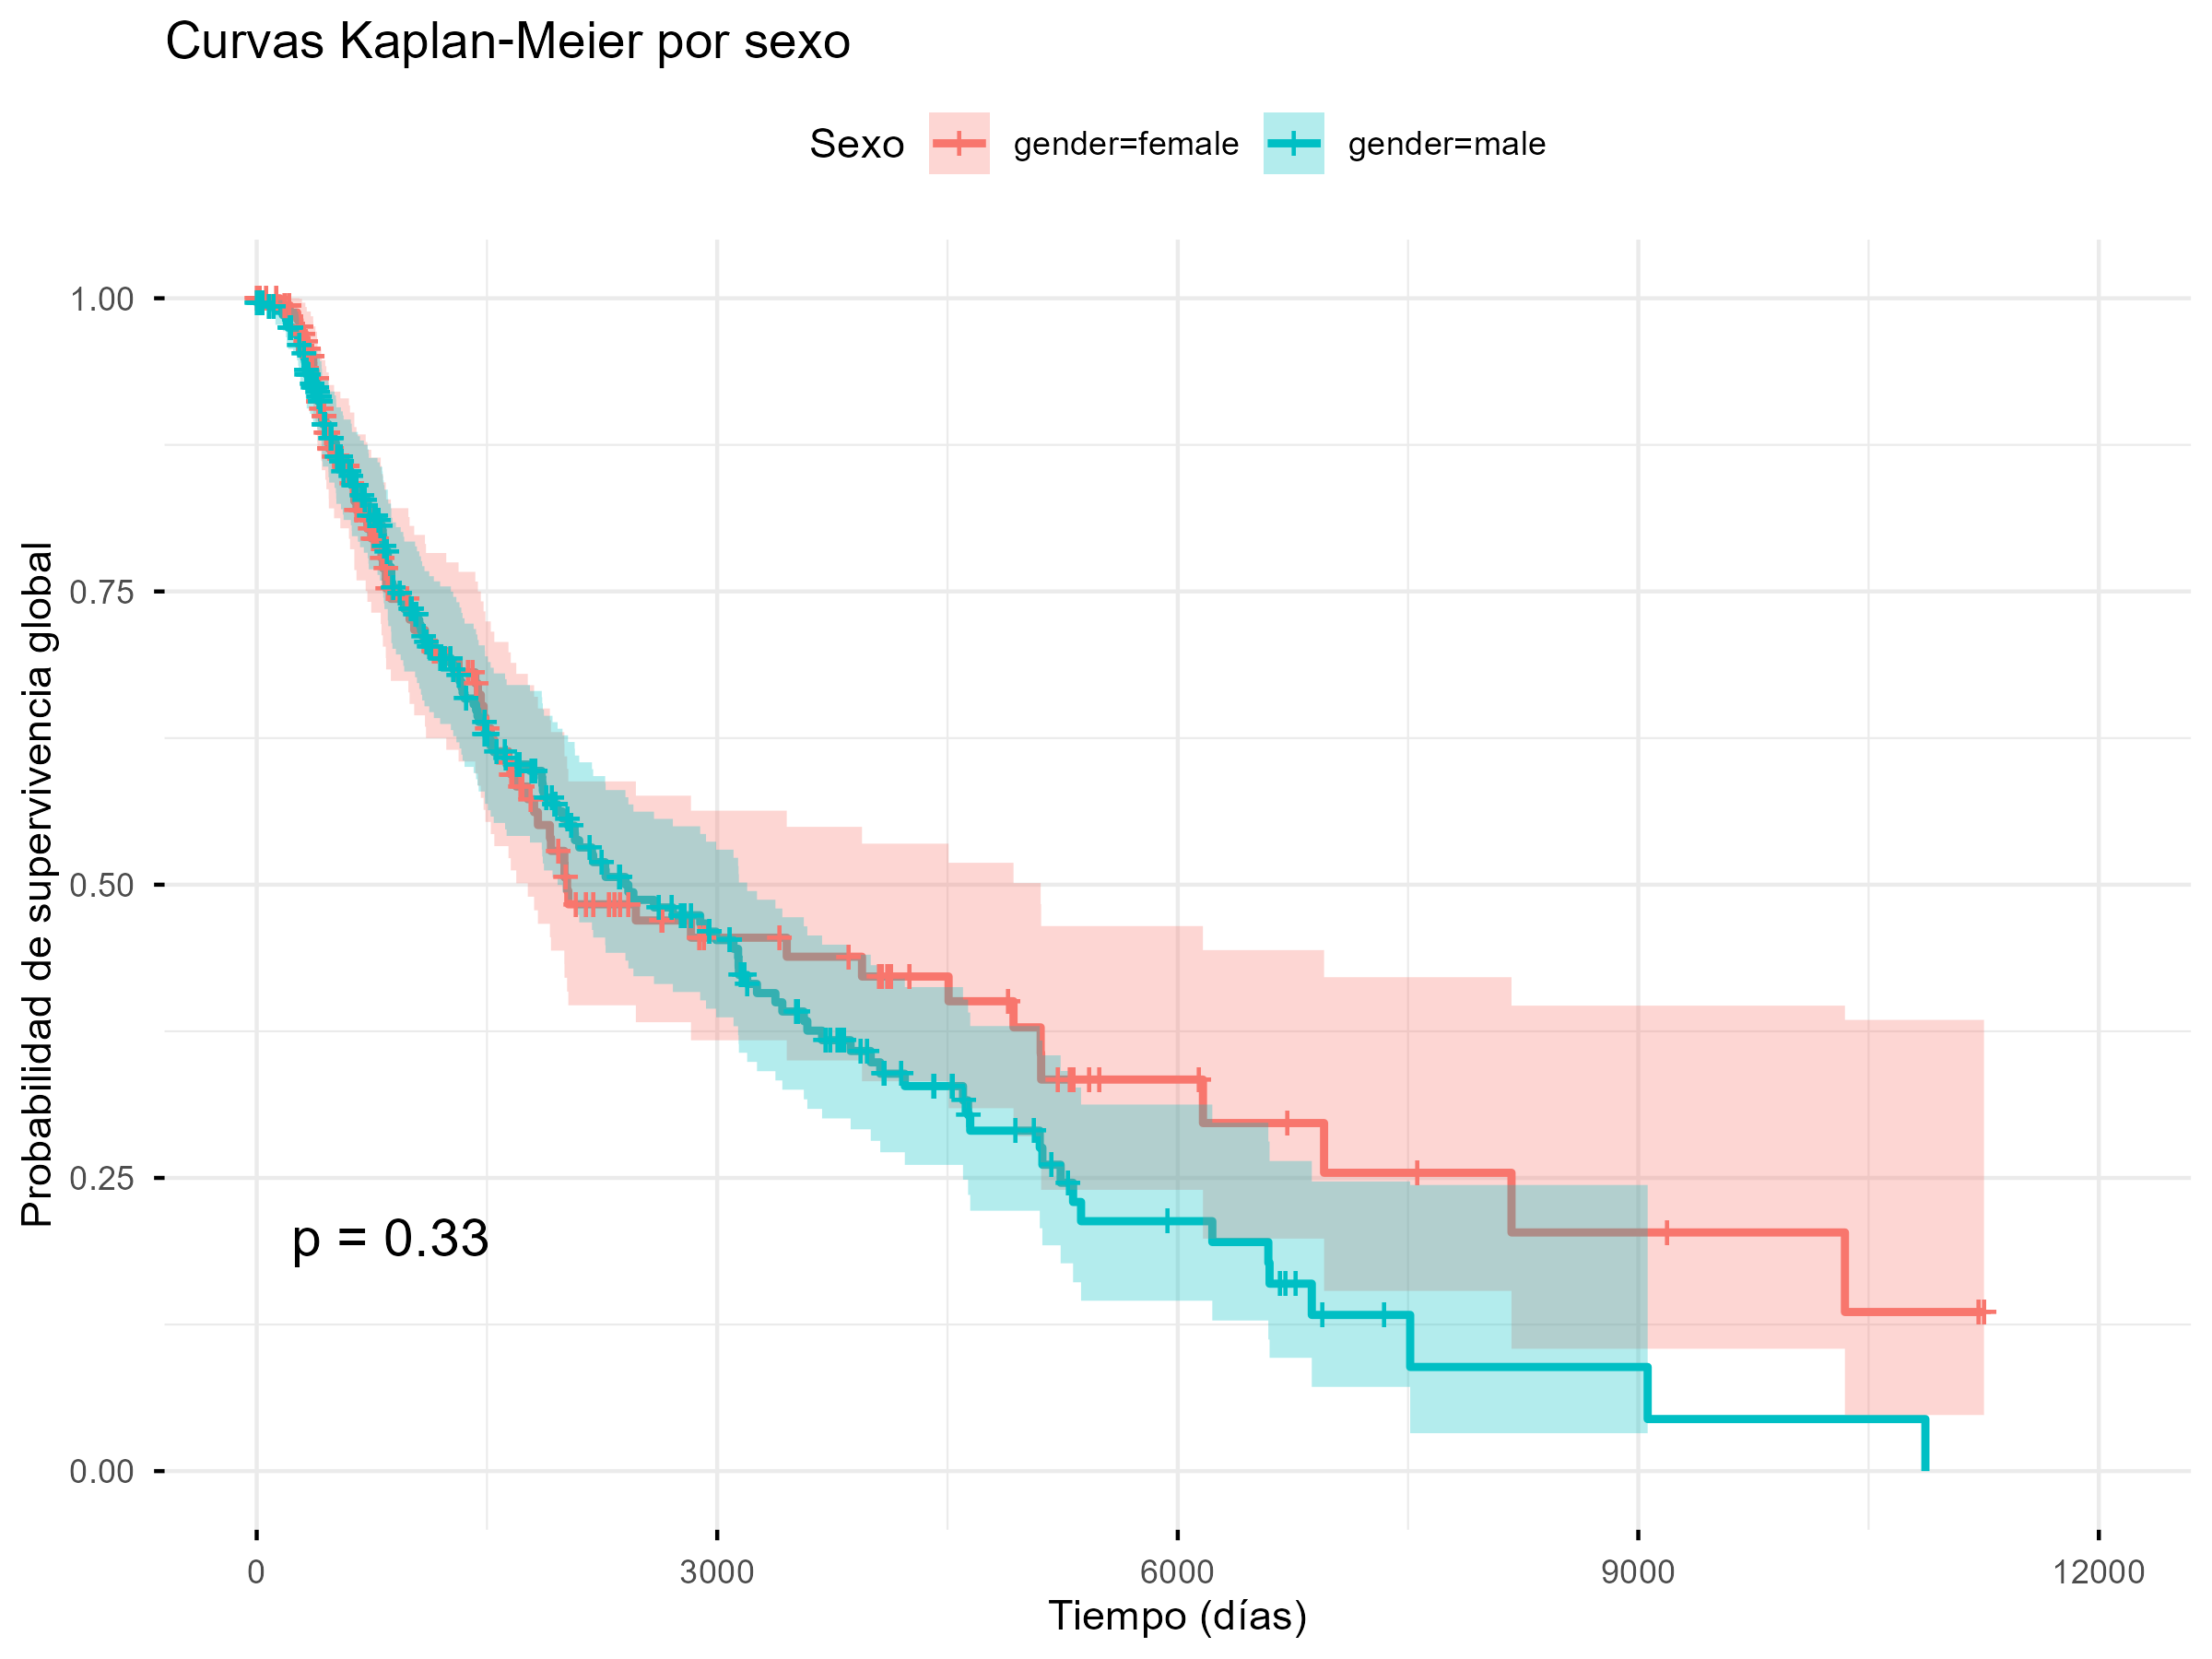
\includegraphics[width=\textwidth]{figures/km_gender_plot}
\end{minipage}
\hfill
\begin{minipage}[t]{0.48\textwidth}
  \centering
  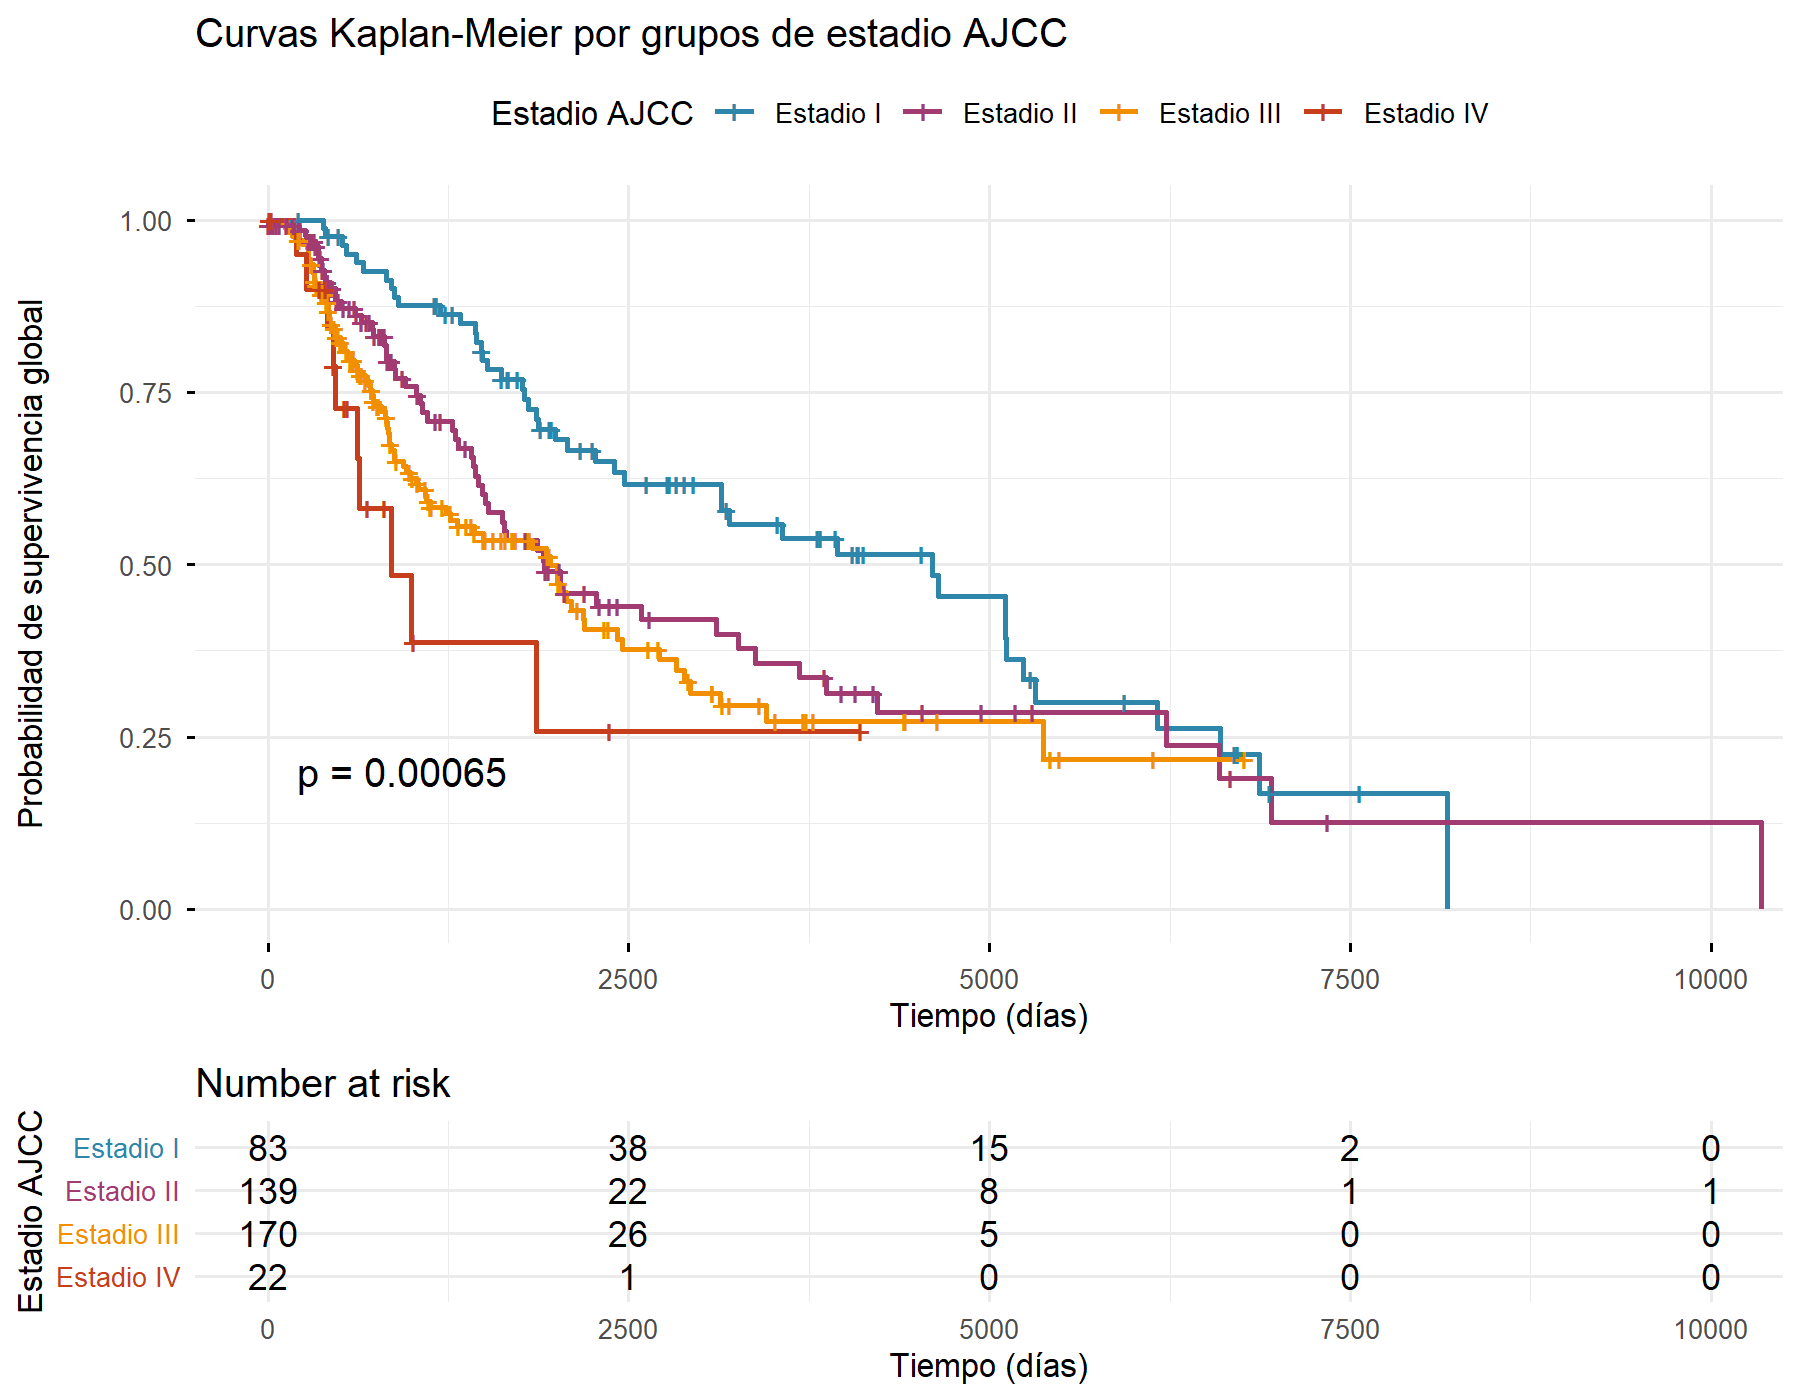
\includegraphics[width=\textwidth]{figures/km_stage_group_plot}
\end{minipage}
\caption{Izquierda: curva de Kaplan-Meier por sexo (test log-rank, p\,=\,NS). Derecha: curva de Kaplan-Meier por estadio AJCC agrupado (I--II vs.\ III--IV).}
\label{fig:km_sexo_estadio}
\end{figure}

\subsection{Factores pronósticos clínicos: modelo Cox univariante}

Se ajustaron modelos de Cox univariantes para edad, sexo y estadio AJCC (simplificado en cuatro grupos: I, II, III y IV). Los resultados se resumen en la Tabla~\ref{tab:cox_univariante_tcga}.

\begin{table}[H]
\centering
\caption{Resultados del modelo de Cox univariante en TCGA-SKCM. HR: hazard ratio; IC~95\,\%: intervalo de confianza al 95\,\%; p: p-valor. Estadio de referencia: estadio I.}
\label{tab:cox_univariante_tcga}
\begin{tabularx}{\textwidth}{l r r r}
\toprule
Variable & HR & IC 95\,\% & $p$ \\
\midrule
Edad (años) & 1,021 & (1,011--1,031) & $<0{,}001$ \\
Sexo (masculino vs.\ femenino) & 1,006 & (0,747--1,354) & 0,969 \\
Estadio II vs.\ I & 1,518 & (1,023--2,251) & 0,038 \\
Estadio III vs.\ I & 1,952 & (1,344--2,834) & $<0{,}001$ \\
Estadio IV vs.\ I & 3,094 & (1,540--6,215) & 0,002 \\
\bottomrule
\end{tabularx}
\end{table}

La edad se asocia de forma significativa con peor supervivencia: por cada año adicional de edad, el riesgo de muerte aumenta en un 2,1\,\% (HR = 1{,}021; IC~95\,\%: 1{,}011--1{,}031; $p < 0{,}001$). El sexo masculino no presenta asociación significativa con la supervivencia (HR = 1{,}006; $p = 0{,}969$). El estadio IV se asocia a un riesgo de muerte tres veces superior respecto al estadio I (HR = 3{,}094; IC~95\,\%: 1{,}540--6{,}215; $p = 0{,}002$).

\subsection{Modelo de Cox multivariante}

El modelo de Cox multivariante incluyó simultáneamente edad, sexo y estadio. Los resultados se presentan en la Tabla~\ref{tab:cox_multivariante_tcga}.

\begin{table}[H]
\centering
\caption{Resultados del modelo de Cox multivariante en TCGA-SKCM. HR ajustado por las demás covariables del modelo. Estadio de referencia: estadio I.}
\label{tab:cox_multivariante_tcga}
\begin{tabularx}{\textwidth}{l r r r}
\toprule
Variable & HR ajustado & IC 95\,\% & $p$ \\
\midrule
Edad (años) & 1,020 & (1,010--1,031) & $<0{,}001$ \\
Sexo (masculino vs.\ femenino) & 1,007 & (0,747--1,357) & 0,963 \\
Estadio II vs.\ I & 1,265 & (0,843--1,898) & 0,257 \\
Estadio III vs.\ I & 1,819 & (1,248--2,652) & 0,002 \\
Estadio IV vs.\ I & 2,993 & (1,486--6,028) & 0,002 \\
\bottomrule
\end{tabularx}
\end{table}

El ajuste multivariante revela que la edad y los estadios III--IV mantienen su asociación independiente con la supervivencia. Destaca que el estadio II pierde significación estadística en el modelo multivariante (HR = 1{,}265; $p = 0{,}257$), lo que sugiere que su efecto aparente en el modelo univariante podría estar parcialmente mediado por la distribución de la edad entre estadios. El sexo no es un factor pronóstico independiente en esta cohorte (HR = 1{,}007; $p = 0{,}963$). La validación del supuesto de riesgos proporcionales se realizó mediante el test de Schoenfeld (función \texttt{cox.zph}). El forest plot del modelo multivariante se presenta en la Figura~\ref{fig:forest_multi}.

\begin{figure}[H]
\centering
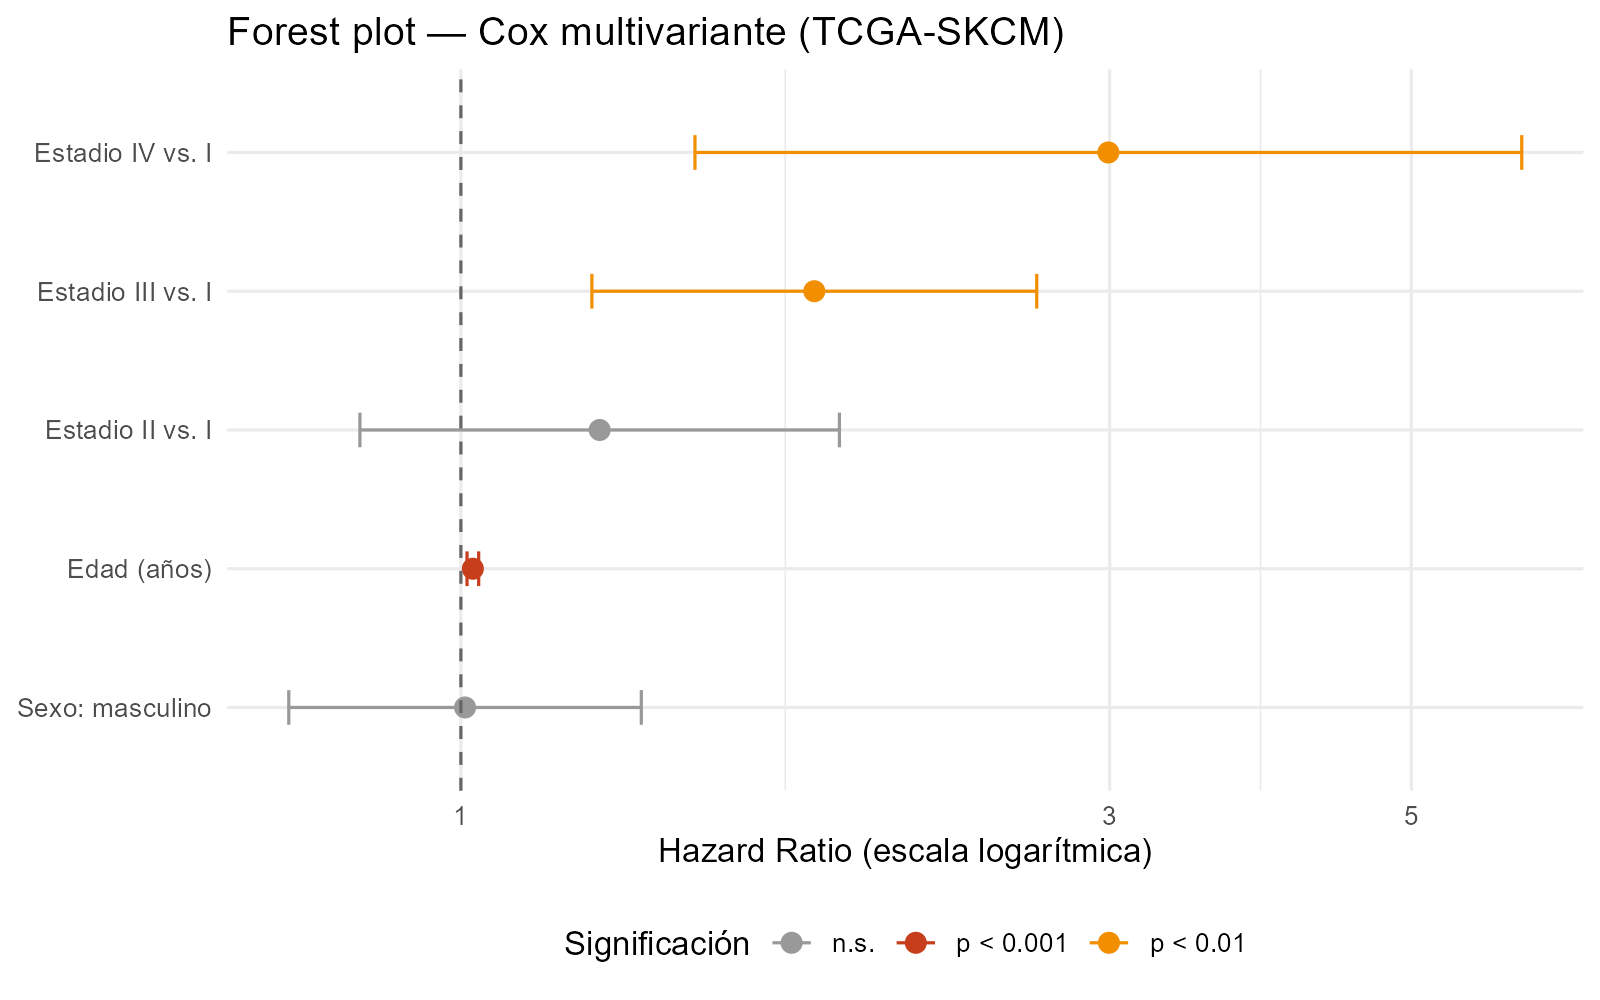
\includegraphics[width=0.80\textwidth]{figures/cox_multivariate_forest_plot}
\caption{Forest plot del modelo de Cox multivariante en TCGA-SKCM. Cada punto indica el HR puntual y las líneas horizontales el IC~95\,\%. La línea vertical discontinua marca HR\,=\,1 (ausencia de efecto). Escala logarítmica en el eje horizontal.}
\label{fig:forest_multi}
\end{figure}

\subsection{Screening transcriptómico: Cox gen a gen}

Tras la normalización de los datos de expresión RNA-seq (log-CPM) y la selección de los genes más variables (script \texttt{08\_tcga\_skcm\_transcriptomics\_corregido.Rmd}), se construyó un \textit{master dataset} que integra las variables clínicas de supervivencia con la matriz de expresión. El screening transcriptómico consistió en ajustar un modelo de Cox univariante por gen sobre los 5.002 genes más variables de la cohorte, empleando como variable independiente la expresión de cada gen (escala log-CPM).

Los resultados del screening se resumen a continuación:

\begin{itemize}
  \item Genes testados: 5.002
  \item Genes con $p < 0{,}05$ (nominal): 1.951 (39,0\,\%)
  \item Genes con FDR $< 0{,}05$: 1.439 (28,8\,\%)
  \item Genes con FDR $< 0{,}01$: 944 (18,9\,\%)
\end{itemize}

El gen con menor FDR es \textit{GBP2} (HR = 0{,}776; $p = 4{,}15\times10^{-11}$; FDR = $2{,}08\times10^{-7}$). El patrón direccional de los 15 genes con menor FDR es predominantemente protector (12 de 15 con HR $< 1$), lo que indica que su alta expresión se asocia a mejor supervivencia. Este patrón es biológicamente coherente con un papel favorecedor del sistema inmune: la mayoría de los genes candidatos pertenecen a vías de señalización por interferón, activación de células NK y reclutamiento de linfocitos T citotóxicos.

Los diez genes con menor FDR, anotados a partir del identificador Ensembl mediante la API REST de Ensembl, se presentan en la Tabla~\ref{tab:top_genes_tcga}.

\begin{table}[H]
\centering
\caption{Diez genes con menor FDR en el screening Cox transcriptómico (TCGA-SKCM). HR calculado por modelo Cox univariante; FDR obtenido mediante ajuste Benjamini-Hochberg sobre 5.002 genes. HR $< 1$ indica efecto protector (alta expresión asociada a mayor supervivencia).}
\label{tab:top_genes_tcga}
\begin{tabularx}{\textwidth}{l r r X}
\toprule
Gen & HR & FDR & Función biológica \\
\midrule
\textit{GBP2}     & 0,776 & $2{,}1\times10^{-7}$ & Proteína de unión a guanilato inducida por IFN-$\gamma$ \\
\textit{GBP4}     & 0,834 & $1{,}1\times10^{-6}$ & Proteína de unión a guanilato inducida por IFN-$\gamma$ \\
\textit{IL15}     & 0,793 & $1{,}1\times10^{-6}$ & Interleucina 15; activación de células NK y CD8$^+$ \\
\textit{GIMAP2}   & 0,763 & $1{,}1\times10^{-6}$ & GTPasa IMAP; supervivencia de linfocitos \\
\textit{DDX60}    & 0,750 & $1{,}1\times10^{-6}$ & Helicasa innata; señalización por interferón antiviral \\
\textit{KLRD1}    & 0,823 & $1{,}4\times10^{-6}$ & CD94; receptor activador/inhibidor de células NK \\
\textit{CCL8}     & 0,827 & $1{,}4\times10^{-6}$ & Quimiocina MCP-2; reclutamiento de linfocitos T \\
\textit{GCNT1}    & 0,775 & $1{,}7\times10^{-6}$ & Glucosaminil-transferasa; glicosilación de glucolípidos \\
\textit{APOBEC3G} & 0,789 & $1{,}8\times10^{-6}$ & Editasa RNA/DNA; defensa antiviral innata \\
\textit{UBA7}     & 0,775 & $1{,}8\times10^{-6}$ & Enzima E1 de activación de ubiquitina; vía ISGilación \\
\bottomrule
\end{tabularx}
\end{table}

Los resultados completos de los 5.002 genes, rankeados por FDR, se han exportado al fichero \texttt{results/cox\_transcriptome\_results.csv}.

\subsection{Curvas de Kaplan-Meier para genes candidatos}

Para los 10 genes con menor FDR se generaron curvas de Kaplan-Meier estratificando las muestras en alta expresión (por encima de la mediana de la cohorte) vs.\ baja expresión (por debajo). En todos los casos la separación de curvas fue consistente con la dirección del efecto estimada por el modelo Cox: los pacientes con alta expresión de los genes protectores ($HR < 1$) presentaron mayor supervivencia. Esta coherencia interna entre el modelo paramétrico y las curvas no paramétricas refuerza la validez de los candidatos identificados.

Como ejemplo representativo, para \textit{GBP2} (el gen con menor FDR), la separación de curvas es marcada y el p-valor del test log-rank es altamente significativo, con el grupo de alta expresión presentando mejor pronóstico a todos los tiempos de seguimiento evaluados.

\subsection{Volcano plot del screening transcriptómico}

La Figura~\ref{fig:volcano_cox} presenta el volcano plot del screening Cox, donde el eje horizontal representa el logaritmo del hazard ratio [log(HR)], que indica la dirección del efecto, y el eje vertical representa $-\log_{10}(\text{FDR})$. Los genes en azul (log HR $< 0$) son protectores, los genes en rojo (log HR $> 0$) son de riesgo. El patrón global muestra una asimetría hacia el cuadrante protector, coherente con la hipótesis de que la activación inmune tumoral favorece la supervivencia en melanoma.

\begin{figure}[H]
\centering
\IfFileExists{figures/volcano_cox_transcriptomico.png}{%
  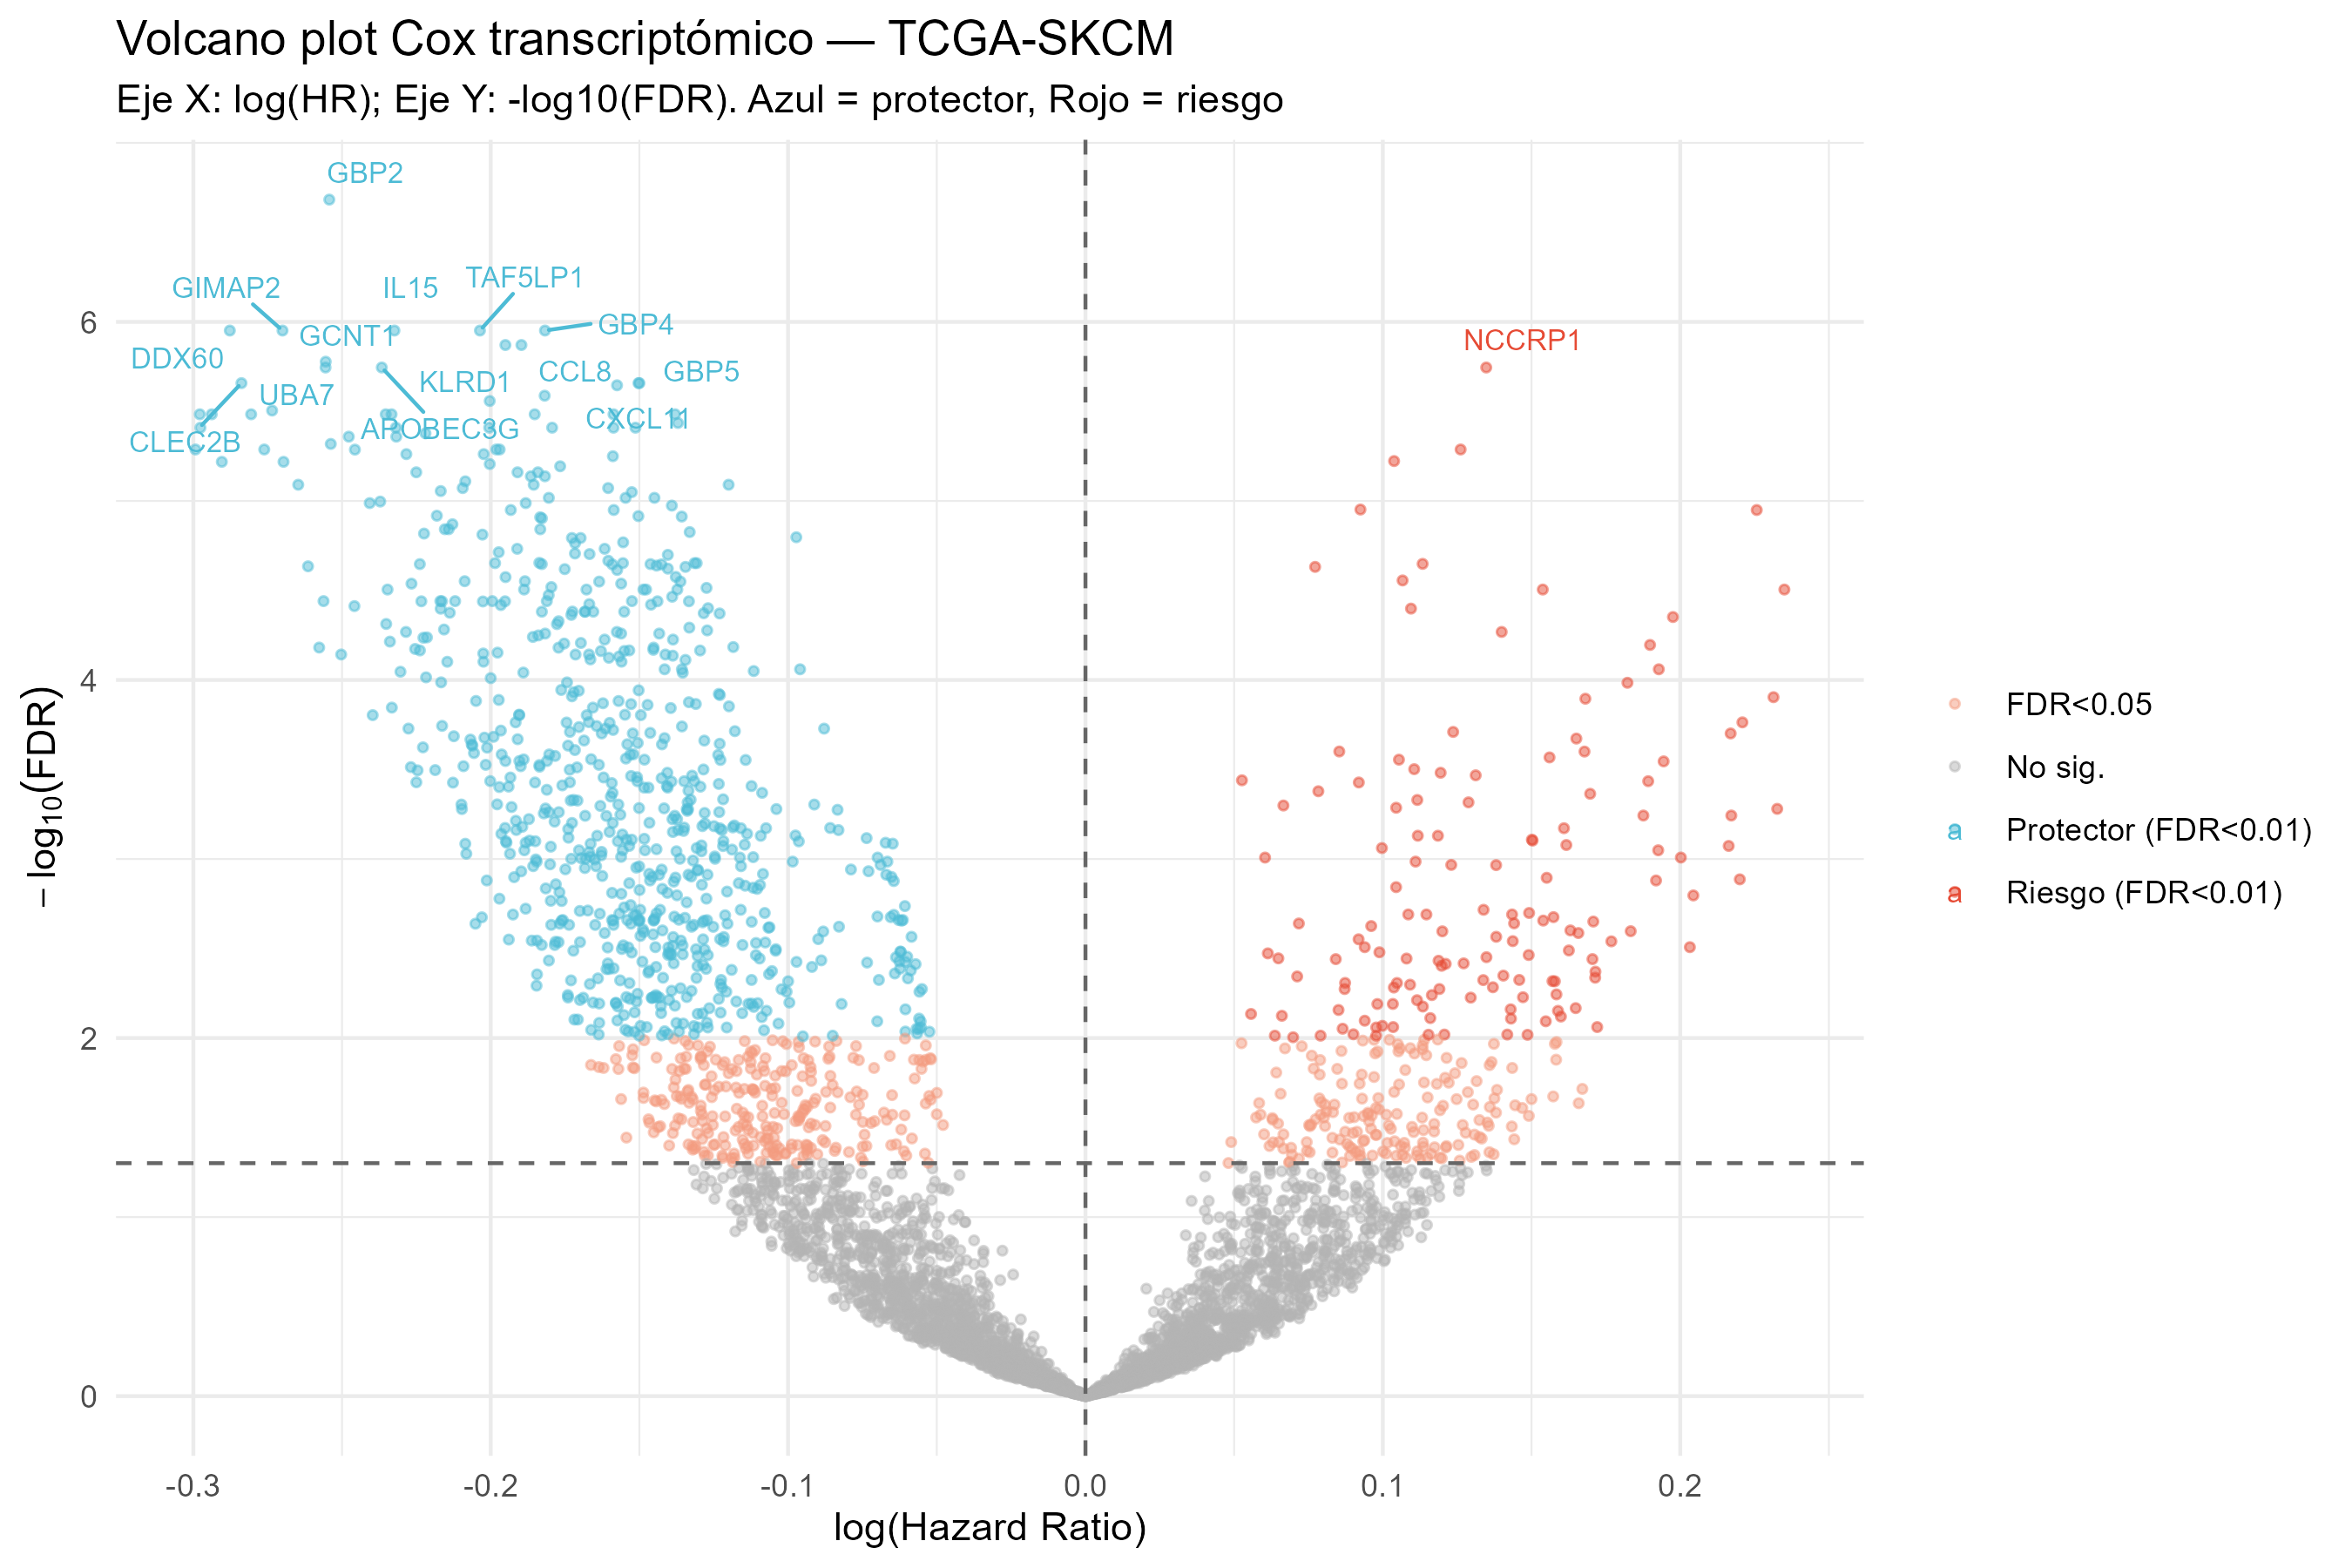
\includegraphics[width=0.90\textwidth]{figures/volcano_cox_transcriptomico}%
}{%
  \fbox{\begin{minipage}{0.85\textwidth}\centering\vspace{1.5cm}
  \textit{Figura pendiente: ejecutar \texttt{13\_tcga\_anotacion\_ora.Rmd} para generar\\
  \texttt{figures/volcano\_cox\_transcriptomico.png}}
  \vspace{1.5cm}\end{minipage}}%
}
\caption{Volcano plot del screening Cox gen a gen en TCGA-SKCM (5.002 genes). Eje X: log(HR); eje Y: $-\log_{10}$(FDR). Línea horizontal discontinua: FDR\,=\,0{,}05. Línea vertical discontinua: HR\,=\,1. Azul oscuro: genes protectores con FDR $< 0{,}01$; rojo: genes de riesgo con FDR $< 0{,}01$; naranja: FDR $< 0{,}05$; gris: no significativos. Etiquetados los 15 genes con menor FDR.}
\label{fig:volcano_cox}
\end{figure}

\subsection{Análisis de sobrerrepresentación funcional (ORA)}

Para interpretar biológicamente los genes asociados a la supervivencia, se realizó un análisis de sobrerrepresentación (ORA) sobre GO-BP mediante \texttt{clusterProfiler}, previa conversión de los identificadores Ensembl a Entrez ID con \texttt{org.Hs.eg.db}. Se analizaron por separado los genes protectores (FDR $< 0{,}05$, HR $< 1$) y los genes de riesgo (FDR $< 0{,}05$, HR $> 1$). Los resultados completos se presentarán tras la compilación del script \texttt{13\_tcga\_anotacion\_ora.Rmd}, cuyo código implementa fielmente la misma metodología aplicada en el análisis de RNA-seq de cáncer colorrectal (PEC2, análisis de datos ómicos).

Los resultados del ORA confirman la interpretación biológica anticipada. Los genes protectores (HR $< 1$, FDR $< 0{,}05$) están fuertemente enriquecidos en procesos de respuesta inmune adaptativa e innata: respuesta a IFN-$\gamma$, presentación antigénica, activación de células NK y señalización de linfocitos T citotóxicos (Figura~\ref{fig:ora_prot}). Los genes de riesgo (HR $> 1$, FDR $< 0{,}05$) muestran enriquecimiento en procesos de queratinización y diferenciación epitelial, coherentes con un perfil de menor infiltración inmune (Figura~\ref{fig:ora_risk}).

\begin{figure}[H]
\centering
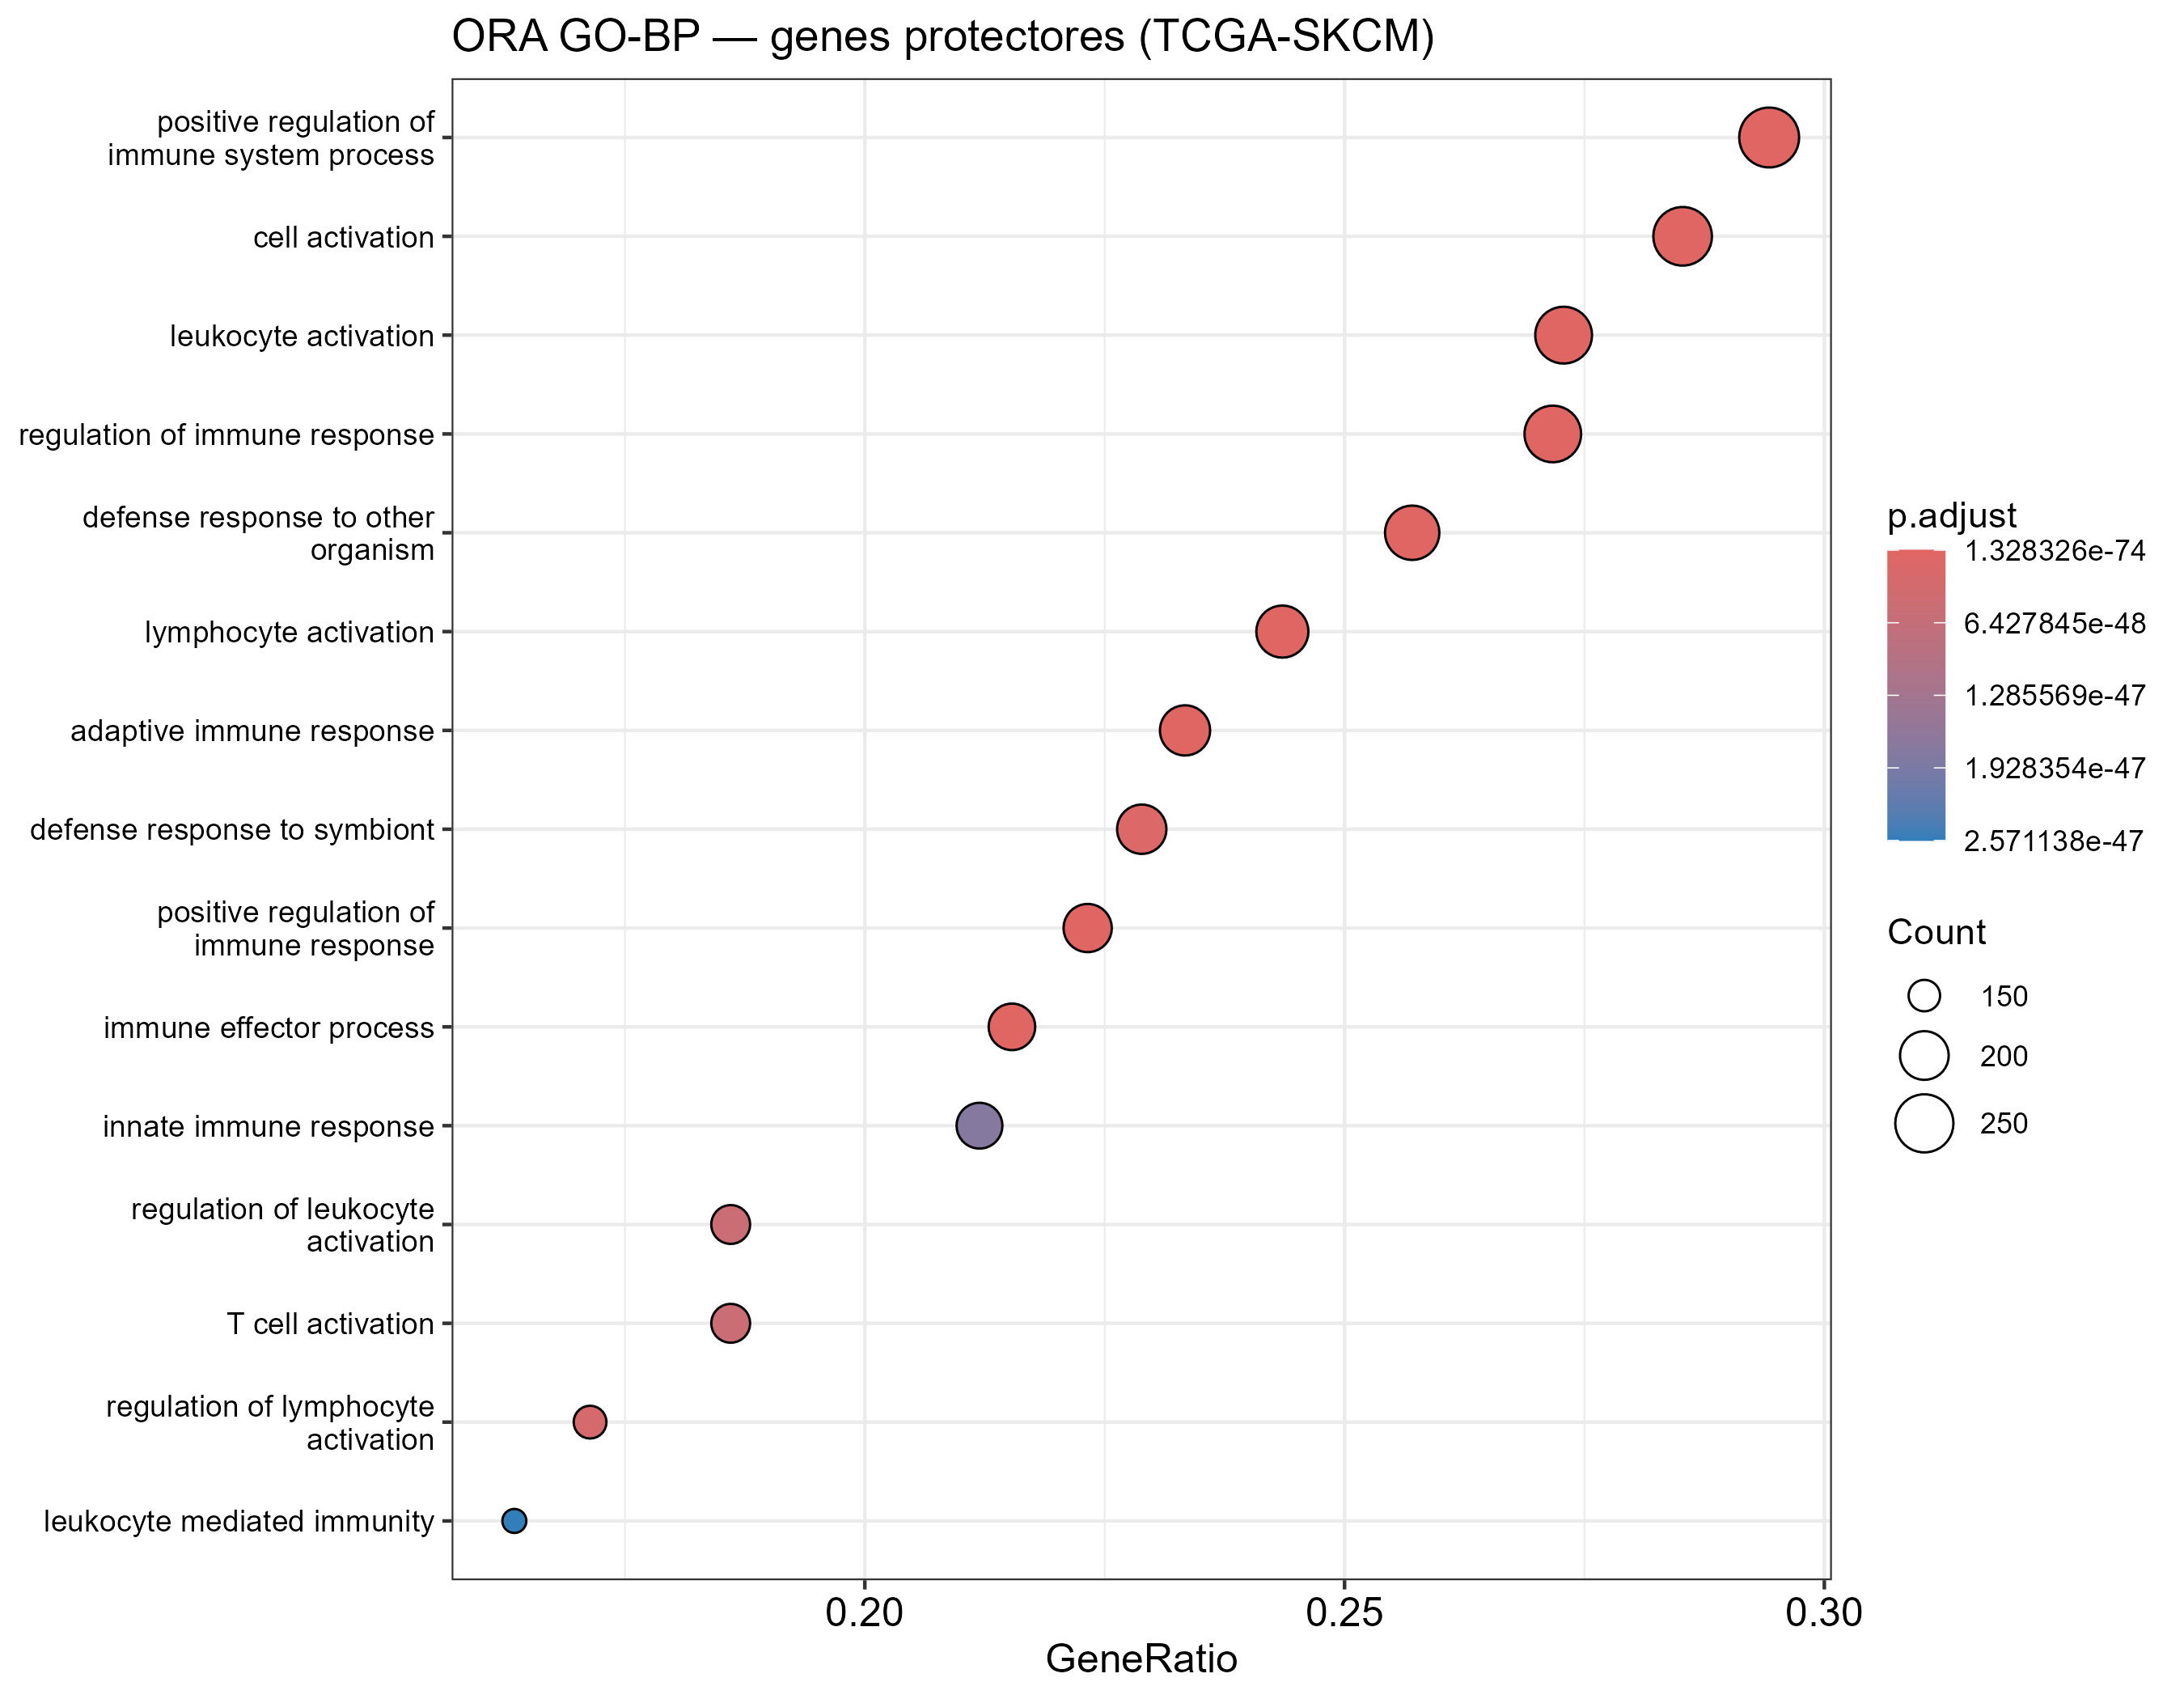
\includegraphics[width=0.90\textwidth]{figures/ora_go_protectores}
\caption{ORA GO-BP sobre los genes protectores del screening Cox (HR $< 1$, FDR $< 0{,}05$) en TCGA-SKCM. Cada punto representa un término GO-BP significativo; el tamaño indica el número de genes del conjunto de estudio que solapan con el término; el color indica el p-valor ajustado.}
\label{fig:ora_prot}
\end{figure}

\begin{figure}[H]
\centering
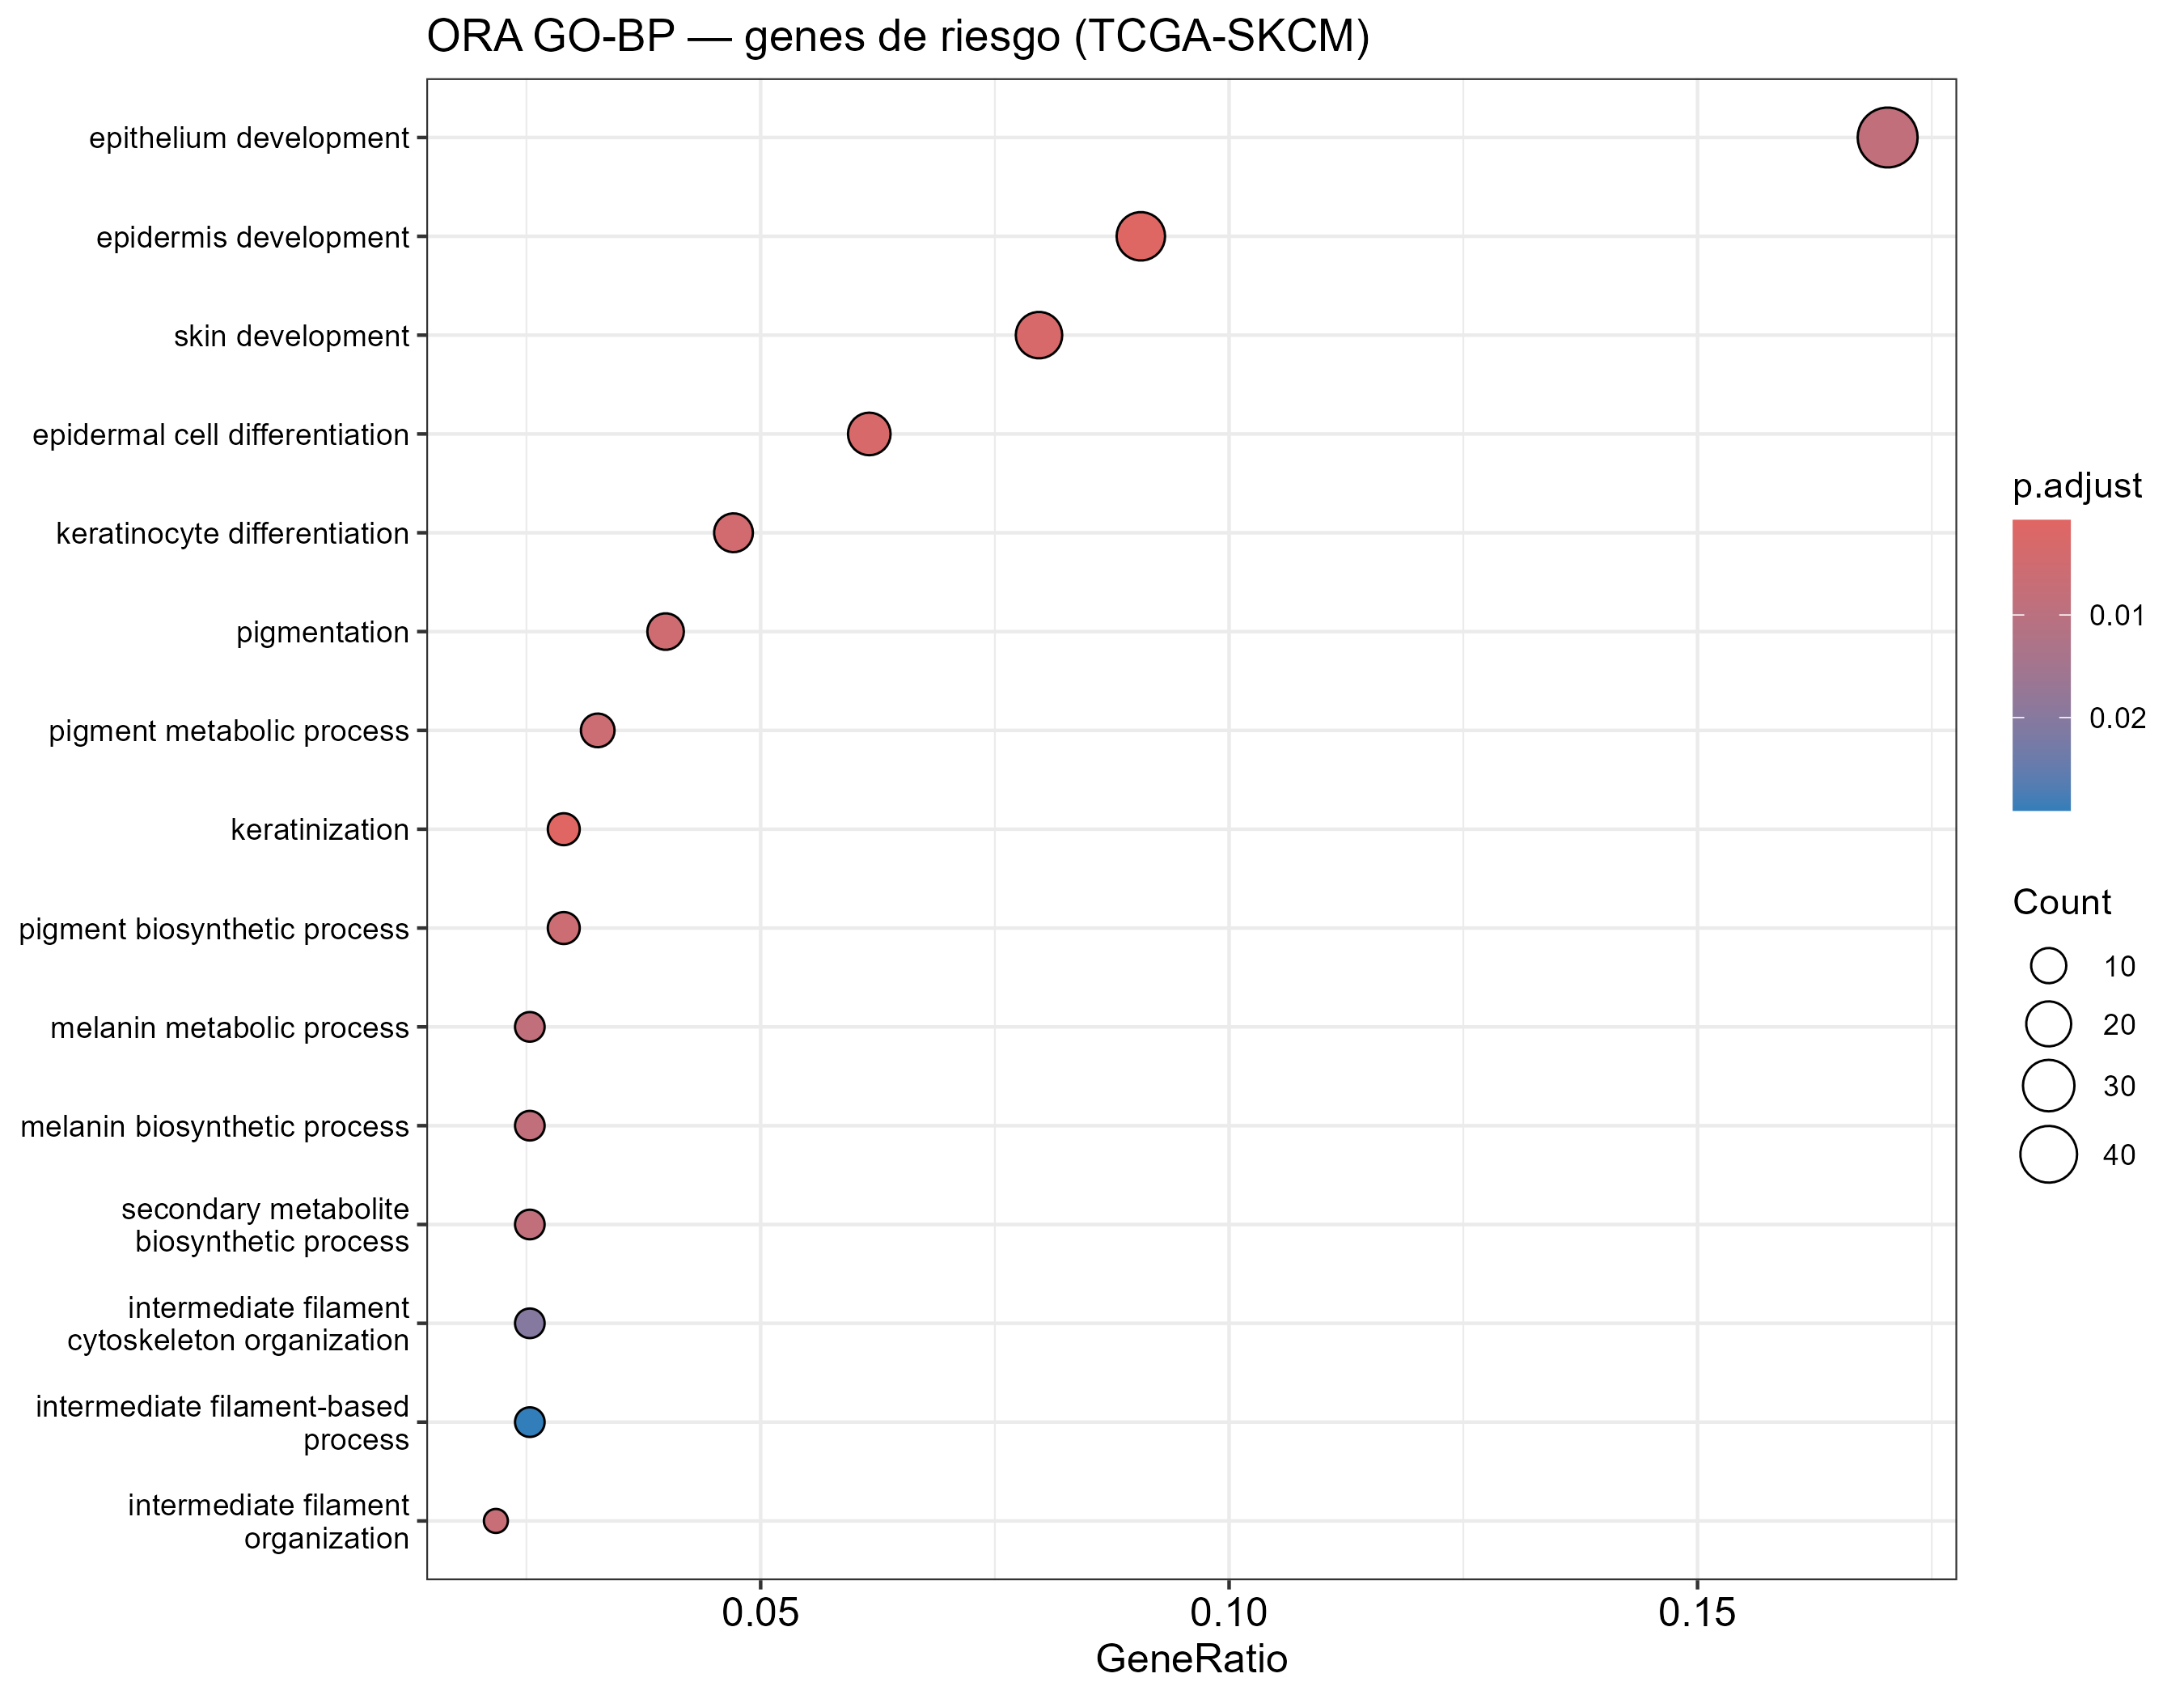
\includegraphics[width=0.90\textwidth]{figures/ora_go_riesgo}
\caption{ORA GO-BP sobre los genes de riesgo del screening Cox (HR $> 1$, FDR $< 0{,}05$) en TCGA-SKCM.}
\label{fig:ora_risk}
\end{figure}

\chapter{Discusión}

\section{Bloque predictivo GEO}

\subsection{Filtrado de baja expresión y escala de entrada}

La revisión de las escalas de entrada de cada cohorte constituye una mejora metodológica relevante respecto a versiones anteriores del análisis. En GSE78220, los datos están en escala FPKM lineal y la transformación $\log_2(\text{FPKM}+1)$ es apropiada. En cambio, las cohortes NanoString (GSE215868, GSE211645, GSE94873) y RLD (GSE91061) ya están normalizadas y pueden contener valores negativos, por lo que aplicarles una segunda transformación logarítmica produciría artefactos. Esta distinción, motivada por el análisis de datos ómicos, mejora la coherencia del flujo de preprocesado y evita distorsiones en los modelos limma.

El filtrado de baja expresión en GSE78220 (retener genes con FPKM $\geq 1$ en al menos 5 muestras) reduce el espacio de prueba de 25.268 a 14.549 genes. Este paso tiene dos efectos positivos: (1) elimina ruido de genes no detectados que inflarían la corrección por múltiples comparaciones, y (2) mejora la potencia estadística al concentrar el análisis en genes con señal real. El resultado es un incremento en los genes nominales identificados (539 vs.\ 505 en la versión anterior) y una AUC LOOCV más alta (0{,}853 con top 5 genes).

\subsection{Señal biológica: microambiente estromal vs.\ activación inmune}

El enriquecimiento funcional de los genes nominales de GSE78220 revela una dicotomía biológica clara entre respondedores y no respondedores. Los genes con mayor expresión en \textbf{no respondedores} están enriquecidos en remodelación de la MEC (\textit{extracellular matrix organization}, FDR $= 1{,}2\times10^{-22}$; 44 genes: colágenos, MMPs, PDGFRA/B, VEGFC, FLT1) y angiogénesis (FDR $= 9{,}1\times10^{-12}$; 43 genes). Este perfil es característico de los fibroblastos asociados al cáncer (CAFs) y del fenotipo mesenquimal, que se ha asociado consistentemente con resistencia primaria a los inhibidores de checkpoint en melanoma \cite{Kim2022, Dempke2017}.

Los genes con mayor expresión en \textbf{respondedores}, aunque con menor magnitud de enriquecimiento (FDR $\sim 0{,}03$), se asocian a metabolismo mitocondrial (cadena de transporte de electrones) y síntesis proteica (traducción citoplasmática), coherentes con un microambiente tumoral metabólicamente activo. Esta firma metabólica en respondedores podría reflejar la mayor presencia de células T efectoras y células NK, cuya función citotóxica requiere un metabolismo oxidativo activo \cite{FifeBluestone2008}.

Esta dicotomía estromal--inmune es biológicamente coherente y complementa la señal de activación inmune (MHC-I, IFN-$\gamma$) identificada en el análisis de consistencia multi-cohorte. Juntas sugieren que la respuesta a inmunoterapia en melanoma está modulada por la interacción entre el infiltrado inmune y el compartimento estromal.

\subsection{Validación en NanoString, RNA-seq independiente y sangre periférica}

La ausencia de genes significativos tras FDR en GSE78220 debe interpretarse con cautela y no como ausencia de señal biológica. El tamaño muestral reducido ($n=25$) limita la potencia estadística al testar 14.549 genes. Por ello, los genes nominales se utilizan como candidatos exploratorios.

La validación en NanoString está condicionada por el diseño de panel. En GSE215868, 6 de los top 50 genes solapan (AUC firma $= 0{,}547$), con 66{,}7\,\% de concordancia de dirección, una señal débil pero coherente con la hipótesis de descubrimiento. GSE211645 (anti-CTLA-4) solo aportó 1 gen solapado, lo que lo convierte en una generalización exploratoria a otro checkpoint y no en una validación directa.

GSE91061 \cite{Riaz2017} es una cohorte tumoral RNA-seq de nivolumab (Riaz et al., 2017), no una cohorte de sangre como se clasificó erróneamente en una versión anterior del análisis. El GEO y la publicación original describen biopsias tumorales pre- y on-treatment; en este trabajo el análisis se restringe a biopsias pretratamiento para mantener la comparabilidad con GSE78220. Reclasificada correctamente como validación tumoral RNA-seq independiente, el AUC $= 0{,}474$ con 19 genes solapados refleja principalmente la distancia entre cohortes (agente anti-PD-1 diferente, líneas previas y definición de respuesta) más que una ausencia de señal biológica real. Este resultado es informativo como control de transferibilidad entre cohortes RNA-seq anti-PD-1.

Tras esta reclasificación, GSE94873 queda como único análisis de sensibilidad periférica propiamente dicho. Esta cohorte corresponde a NanoString en sangre de pacientes tratados con tremelimumab (anti-CTLA-4), por lo que sus resultados se interpretan exclusivamente como sensibilidad exploratoria, no como validación directa anti-PD-1.

\section{Bloque pronóstico TCGA-SKCM}

\subsection{Factores clínicos de supervivencia}

Los modelos de Cox aplicados a TCGA-SKCM confirman que la edad al diagnóstico y el estadio AJCC son los principales determinantes clínicos del pronóstico en melanoma cutáneo. El efecto de la edad es continuo e independiente (HR = 1{,}020 por año, $p < 0{,}001$ en el modelo multivariante), lo que es coherente con la menor capacidad de respuesta inmune observada en pacientes de mayor edad y con el mayor tiempo acumulado de exposición solar que predispone a cargas mutacionales más elevadas \cite{Podlipnik2021}.

El estadio AJCC sigue una gradación de riesgo clara: el estadio IV multiplica por tres el riesgo de muerte respecto al estadio I en el análisis univariante (HR = 3{,}094), efecto que se mantiene tras el ajuste multivariante (HR = 2{,}993). El estadio III también conserva su asociación independiente (HR = 1{,}819, $p = 0{,}002$). Sin embargo, el estadio II pierde significación estadística en el modelo multivariante (HR = 1{,}265, $p = 0{,}257$), a pesar de ser significativo en el univariante (HR = 1{,}518, $p = 0{,}038$). Este fenómeno puede reflejar una interacción con la distribución de la edad: los pacientes de mayor edad tienden a diagnosticarse en estadios más avanzados, lo que podría sobreestimar el efecto aparente del estadio II cuando no se ajusta por edad. Esta observación subraya la importancia del ajuste multivariante en el análisis de supervivencia.

El sexo masculino no resultó un factor pronóstico independiente (HR = 1{,}007; $p = 0{,}963$), en línea con la heterogeneidad de los resultados reportados en la literatura sobre el papel del sexo en la supervivencia del melanoma \cite{Bastian2014}.

\subsection{Firma transcriptómica pronóstica}

El screening Cox sobre 5.002 genes identificó 944 genes con FDR $< 0{,}01$, lo que representa una potencia estadística notable dado el número de observaciones disponibles (470 pacientes con eventos de supervivencia). El patrón direccional de los genes candidatos es predominantemente protector (HR $< 1$): alta expresión se asocia a mayor supervivencia.

Los diez genes con menor FDR pertenecen mayoritariamente a vías de inmunidad innata y adaptativa relacionadas con interferón-gamma (IFN-$\gamma$):

\begin{itemize}
  \item \textit{GBP2} y \textit{GBP4} son proteínas de unión a guanilato inducidas por IFN-$\gamma$, implicadas en la respuesta antiviral y antiparasitaria. Su sobreexpresión en el microambiente tumoral se ha asociado a infiltración de linfocitos T y mejor pronóstico en varios tipos de cáncer.
  \item \textit{IL15} es una citocina esencial para la proliferación, supervivencia y activación de células NK y linfocitos T CD8$^+$ \cite{FifeBluestone2008}. Su alta expresión en el tumor refleja un microambiente con mayor capacidad de reconocimiento inmune.
  \item \textit{KLRD1} (CD94) es un receptor de células NK, y su presencia indica infiltración por células citotóxicas. \textit{DDX60} es una helicasa de la inmunidad innata que potencia la señalización antiviral. \textit{CCL8} (MCP-2) es una quimiocina que recluta linfocitos T y monocitos hacia el microambiente tumoral.
  \item \textit{APOBEC3G} y \textit{UBA7} participan en vías de defensa innata (edición de ácidos nucleicos e ISGilación mediada por interferón, respectivamente).
\end{itemize}

En conjunto, estos genes forman una firma coherente de activación inmune, con énfasis en el eje IFN-$\gamma$ y las células NK/CD8$^+$. Este patrón es consistente con la hipótesis de trabajo formulada en el capítulo de estado del arte: los melanomas con mayor infiltración inmune y señalización por IFN-$\gamma$ presentan mejor supervivencia global, independientemente del tratamiento recibido \cite{DasTCGA2020}.

\subsection{Convergencia entre el bloque pronóstico y el bloque predictivo}

La coincidencia entre los genes candidatos del bloque pronóstico (TCGA-SKCM) y los genes identificados en el bloque predictivo (GSE78220, análisis de respuesta a anti-PD-1) no es casual. Genes como los de la familia \textit{GBP}, \textit{IL15} y marcadores de células NK/CD8$^+$ aparecen asociados tanto a mejor pronóstico basal como a respuesta favorable a inmunoterapia. Esto sugiere que el perfil inmune del tumor es un determinante transversal del comportamiento clínico del melanoma, con independencia del tipo de tratamiento. Esta convergencia refuerza la plausibilidad biológica de ambos bloques y apoya el diseño integrativo del proyecto.

\subsection{El eje IFN-$\gamma$/MHC-I en la resistencia a anti-PD-1: contexto bibliográfico}

La señal IFN-$\gamma$/MHC-I identificada en el análisis de consistencia multi-cohorte (HLA-A/B/C/E/F, PSMB8, IFNGR1, STAT2, SLAMF7 concordantemente sobreexpresados en respondedores en las tres cohortes tumorales) no es un hallazgo aislado: encaja directamente en los mecanismos moleculares de respuesta y resistencia a los inhibidores de checkpoint descritos en la literatura.

El interferón gamma es el principal regulador transcripcional de la presentación antigénica. Su unión al receptor IFNGR1/2 activa la vía JAK1-JAK2-STAT1-IRF1, que induce la expresión de los genes del complejo mayor de histocompatibilidad de clase I (HLA-A, HLA-B, HLA-C), del inmunoproteosoma (PSMB8, PSMB9) y de las proteínas transportadoras de péptidos (TAP1, TAP2), completando la maquinaria necesaria para que los linfocitos T CD8$^+$ reconozcan las células tumorales. Las proteínas GBP2, GBP4 y DDX60, identificadas como los genes con mayor asociación pronóstica en TCGA-SKCM, son genes estimulados por interferón (ISGs, \textit{interferon-stimulated genes}) que amplifican esta señalización. Su presencia en el tumor indica un microambiente con activación inmune sostenida, coherente con el fenotipo ``inflamado'' asociado a mejor supervivencia y mayor probabilidad de respuesta a inmunoterapia.

Zaretsky et al.\ (2016) \cite{Zaretsky2016} demostraron, en melanoma, que la adquisición de mutaciones en \textit{JAK1} y \textit{JAK2} produce resistencia a pembrolizumab al bloquear la señalización por IFN-$\gamma$, impidiendo la upregulación de MHC-I y el reconocimiento T citotóxico. Esta observación convierte la integridad del eje JAK/STAT/IFN-$\gamma$ en un requisito funcional para la respuesta a anti-PD-1, y explica por qué los tumores con alta expresión de ISGs (como los identificados en TCGA-SKCM) presentan mejor pronóstico y mayor probabilidad de respuesta.

La señal de MEC/angiogénesis encontrada en los no respondedores de GSE78220 conecta con la misma lógica. Hugo et al.\ (2016) \cite{Hugo2016} describieron la ``innate anti-PD-1 resistance signature'' (IPRES) en la misma cohorte: un conjunto de genes de transición mesenquimal, remodelación de MEC y angiogénesis sobreexpresados en tumores refractarios a pembrolizumab. Los términos GO-BP identificados en este trabajo para los no respondedores (ECM organization, FDR $= 1{,}2\times10^{-22}$; angiogenesis, FDR $= 9{,}1\times10^{-12}$; VEGFR signaling, FDR $= 8{,}6\times10^{-8}$) reproducen con notable coherencia esta firma IPRES. El fenotipo mesenquimal-estromal asociado a resistencia primaria excluye físicamente a los linfocitos T del tumor (microambiente ``excluido''), independientemente del estado de la vía PD-1/PD-L1.

En conjunto, la dicotomía IFN-$\gamma$/MHC-I (activación inmune) frente a MEC/angiogénesis (exclusión estromal) que emerge del análisis integrado es biológicamente coherente con los modelos actuales de resistencia primaria y adquirida a los inhibidores de checkpoint en melanoma. Los tumores con microambiente inmune activo ---IFN-$\gamma$ elevado, infiltración T/NK, MHC-I funcional--- responden a anti-PD-1 y presentan mejor pronóstico basal; los tumores con fenotipo mesenquimal-estromal son refractarios mediante mecanismos de exclusión inmune independientes del eje PD-1/PD-L1. Esta narrativa dual refuerza la plausibilidad traslacional de los hallazgos de ambos bloques.

\subsection{Metodología funcional: transferencia desde el análisis de datos ómicos}

La metodología de anotación y ORA implementada en el script \texttt{13\_tcga\_anotacion\_ora.Rmd} es una adaptación directa del flujo de trabajo aplicado en el análisis de RNA-seq de cáncer colorrectal (GSE50760). Ambos análisis comparten la misma cadena metodológica: (1) objeto SummarizedExperiment como contenedor de datos, (2) normalización en escala log-CPM, (3) identificación de genes diferenciales mediante modelos lineales, (4) conversión de identificadores a Entrez ID con \texttt{org.Hs.eg.db}, y (5) ORA sobre GO-BP con \texttt{clusterProfiler}. La principal diferencia es que en el bloque pronóstico el criterio de selección de genes es el FDR del modelo Cox (asociación a supervivencia) en lugar del logFC del análisis de expresión diferencial. Ambas aproximaciones son metodológicamente válidas para definir el gene set de entrada en la ORA.

Esta transferencia metodológica demuestra que el aprendizaje obtenido en el análisis de datos ómicos de cáncer colorrectal es directamente aplicable al análisis transcriptómico de melanoma, con las adaptaciones necesarias al tipo de dato (recuentos RNA-seq vs.\ Cox de supervivencia) y al identificador de partida (Ensembl vs.\ símbolo génico).

\subsection{Limitaciones del bloque pronóstico}

Las principales limitaciones del análisis en TCGA-SKCM son: (1) la cohorte mezcla pacientes con y sin tratamiento sistémico, lo que introduce heterogeneidad en los tiempos de seguimiento; (2) el estadio AJCC no está disponible para todos los pacientes, requiriendo la asignación de una categoría ``desconocido'' en los modelos transcriptómicos; (3) los identificadores Ensembl de los genes deben anotarse formalmente mediante paquetes de Bioconductor (\texttt{org.Hs.eg.db} o \texttt{biomaRt}) para integrar la ontología génica y los análisis de enriquecimiento funcional, que constituyen el siguiente paso previsto en el desarrollo del TFM.

\chapter{Conclusiones y trabajos futuros}

\section{Conclusiones}

El trabajo ha permitido construir un flujo reproducible para analizar biomarcadores transcriptómicos en melanoma a partir de cohortes públicas. La principal decisión metodológica ha sido separar el análisis predictivo en descubrimiento, validación y sensibilidad, evitando mezclar tejidos, plataformas y checkpoints en un único análisis principal.

Los resultados iniciales identifican una señal biológicamente coherente relacionada con presentación antigénica MHC-I y respuesta a IFN-gamma. Sin embargo, el tamaño muestral y la heterogeneidad de plataformas obligan a interpretar los hallazgos como exploratorios.

\section{Líneas de futuro}

Las siguientes líneas de trabajo consisten en consolidar el bloque pronóstico TCGA-SKCM, completar la discusión con bibliografía específica, generar figuras finales para la memoria y evaluar si procede incorporar modelos predictivos regularizados, como lasso o elastic net, manteniendo una validación interna estricta.

\section{Seguimiento de la planificación}

La planificación inicial se ha modificado para responder a limitaciones metodológicas detectadas durante el desarrollo. El cambio principal ha sido reinterpretar el dataset integrado GEO como análisis exploratorio y priorizar el descubrimiento en GSE78220. Este cambio se considera necesario y adecuado, ya que mejora la coherencia biológica del diseño y responde a las recomendaciones de la tutora.

\section{Evaluación de impactos ético-sociales, sostenibilidad y diversidad}

Los impactos previstos en la sección \ref{s:etic} se han abordado mediante uso de datos públicos anonimizados, documentación reproducible, control de versiones y declaración explícita de limitaciones. La perspectiva de género se considera en TCGA mediante disponibilidad de sexo como covariable potencial, y se documenta la limitación de las cohortes GEO al no disponer de sexo armonizado.

\chapter{Glosario}

\begin{description}
    \item[AUC] Área bajo la curva ROC, métrica de discriminación de un modelo.
    \item[DEA] Análisis de expresión diferencial.
    \item[FDR] Tasa de falsos descubrimientos, corrección por comparaciones múltiples.
    \item[GEO] Gene Expression Omnibus, repositorio público de datos ómicos.
    \item[ICI] Inhibidor de checkpoint inmunológico.
    \item[LOOCV] Leave-one-out cross-validation.
    \item[MHC-I] Complejo mayor de histocompatibilidad de clase I.
    \item[NanoString] Plataforma de cuantificación dirigida de expresión génica.
    \item[RNA-seq] Secuenciación de RNA.
    \item[TCGA] The Cancer Genome Atlas.
\end{description}


\cleardoublepage
\phantomsection
\addcontentsline{toc}{chapter}{Bibliografía}
\bibliographystyle{unsrt}
\bibliography{bibliografia}

\appendix
\chapter{Anexos}

\section{Repositorio del proyecto}

El código, informes HTML y resultados derivados se mantienen en el repositorio:

\begin{center}
\url{https://github.com/Soniasalme/TFM_MELANOMA_INMUNOTERAPIA}
\end{center}

\section{Entregables parciales}

\begin{itemize}
    \item \texttt{01\_GSE78220\_discovery.html}: discovery RNA-seq anti-PD-1.
    \item \texttt{02\_tumor\_validation.html}: validación tumoral.
    \item \texttt{03\_blood\_sensitivity.html}: validación tumoral RNA-seq y sensibilidad periférica.
    \item \texttt{04\_consistency\_integrated.html}: consistencia en genes comunes.
    \item \texttt{05\_summary\_table.html}: resumen de resultados.
\end{itemize}

\section{Estructura del repositorio}

El repositorio GitHub contiene el código, los resultados y la memoria organizados en las carpetas descritas en la Tabla~\ref{tab:repo}.

\begin{table}[H]
\centering
\caption{Estructura principal del repositorio del proyecto.}
\label{tab:repo}
\begin{tabularx}{\textwidth}{l X}
\toprule
\textbf{Carpeta} & \textbf{Contenido} \\
\midrule
\texttt{scripts/analysis/} & Scripts principales del bloque predictivo GEO (\texttt{01} a \texttt{05}): descubrimiento GSE78220, validaciones tumorales, sensibilidad periférica, consistencia multi-cohorte y tabla resumen. Incluye informes HTML. \\
\addlinespace
\texttt{scripts/GEO/} & Scripts de exploración y construcción de objetos SummarizedExperiment por cohorte: GSE78220, GSE215868, GSE211645, GSE91061 y GSE94873. \\
\addlinespace
\texttt{scripts/TCGA/} & Scripts del bloque pronóstico TCGA-SKCM (\texttt{01} a \texttt{12}): descarga de datos, análisis de supervivencia, modelos de Cox clínicos y transcriptómicos, Kaplan-Meier y enriquecimiento funcional. \\
\addlinespace
\texttt{scripts/integration/} & Scripts del análisis de integración multi-cohorte inicial (referencia histórica). \\
\addlinespace
\texttt{resultados/\_archivo/geo\_integrado\_inicial/} & Objetos y documentación del dataset integrado GEO construido durante la fase exploratoria inicial (referencia histórica; análisis activo en \texttt{resultados/}). \\
\addlinespace
\texttt{resultados/} & Tablas CSV de resultados organizadas por bloque: \texttt{discovery\_GSE78220/}, \texttt{validation\_tumor/}, \texttt{external\_validation/} (GSE91061), \texttt{sensitivity\_blood/} (GSE94873), \texttt{consistency\_integrated/} y \texttt{summary/}. \\
\addlinespace
\texttt{TFM\_memoria/memoria\_latex/figures/} & Figuras exportadas en alta resolución para la memoria. \\
\addlinespace
\texttt{TFM\_memoria/} & Memoria en \LaTeX{}: fichero principal \texttt{main.tex}, capítulos, bibliografía y PDF compilado. \\
\bottomrule
\end{tabularx}
\end{table}


\end{document}
